\chapter{Experimentelle Resultate und Analysen}
\label{chapter:experiment}

Alle Fits werden durch eine least-squares-Methode erstellt. ***

\section{$T_1$} \label{section:res:T_1}

Vor dem Beginn jeder NMR-Messung ist es sinnvoll, $T_1$ im zu untersuchenden Temperaturgebiet zu vermessen. Dies ist hilfreich um wichtige Parameter der Messungen abzustecken und mögliche Hindernisse im Vorhinein erahnen zu können. So sollte zwischen allen Messungen eine Zeit von mindestens $4 T_1$ gewartet werden, um sicherzugehen, dass sich die Magnetisierung in guter Näherung wieder im Gleichgewichtszustand befindet. Wird $T_1$ also im Laufe der Messung bei anderen Temperaturen länger, muss hierauf Rücksicht genommen werden. Wird $T_1$ auf der anderen Seite sehr kurz, kann es passieren, dass Signale sehr schnell zerfallen und den Experimentierenden mit einem schlechten Signal-Rausch-Verhältnis zurücklassen. Hinzu kommt, dass der Verlauf von $T_1$ nach Formel *** wertvolle Information über die Dynamik in der untersuchten Probe liefern kann. Zuletzt bietet diese recht einfache und reproduzierbare Messung die Möglichkeit, den Aufbau und die Probe auf Übereinstimmung mit Literaturdaten hin zu überprüfen. Daher wurden zu allen untersuchten Temperaturen $T_1$-Messungen aufgenommen.

Zur Bestimmung von $T_1$ wurde eine Invertierungs-Pulsfolge mit Hahn-Echo verwendet. Dabei war die Evolutionszeit $t_p = \SI{15}{\micro s}$.

Aufgenommen am OBI ($\SI{300}{MHz}$) mit Länge eines Pi-Pulses $\tau = \SI{7.6}{\micro s}$. Larmorfrequenz überall $\omega_L = 2 \pi \cdot \SI{97.1722}{MHz}$, sofern nicht anders notiert. ***

Aufgenommen am Bruker ***  Neben dem $\SI{300}{MHz}$-Spektrometer wurden auch einige Messungen an einem $\SI{400}{MHz}$ Spektrometer von Bruker durchgeführt.


Repräsentative Rohdaten einer solchen Messung sind in Abbildung \ref{fig:res:T_1_roh} zu sehen. An die Daten wurden Fits mit $T_1$ und $\beta$ als freien Parametern entsprechend Gleichung \eqref{eqn:theo:T_2_fit} angelegt -- diese sind als Linien dargestellt. Die Daten wurden hier zudem auf den Bereich zwischen $1$ und $-1$ normiert, um einen besseren Vergleich zuzulassen. Es ist zu erkennen, dass die Fits eine gute Repräsentation der Daten ermöglichen.
\begin{figure}
	\begin{center}
		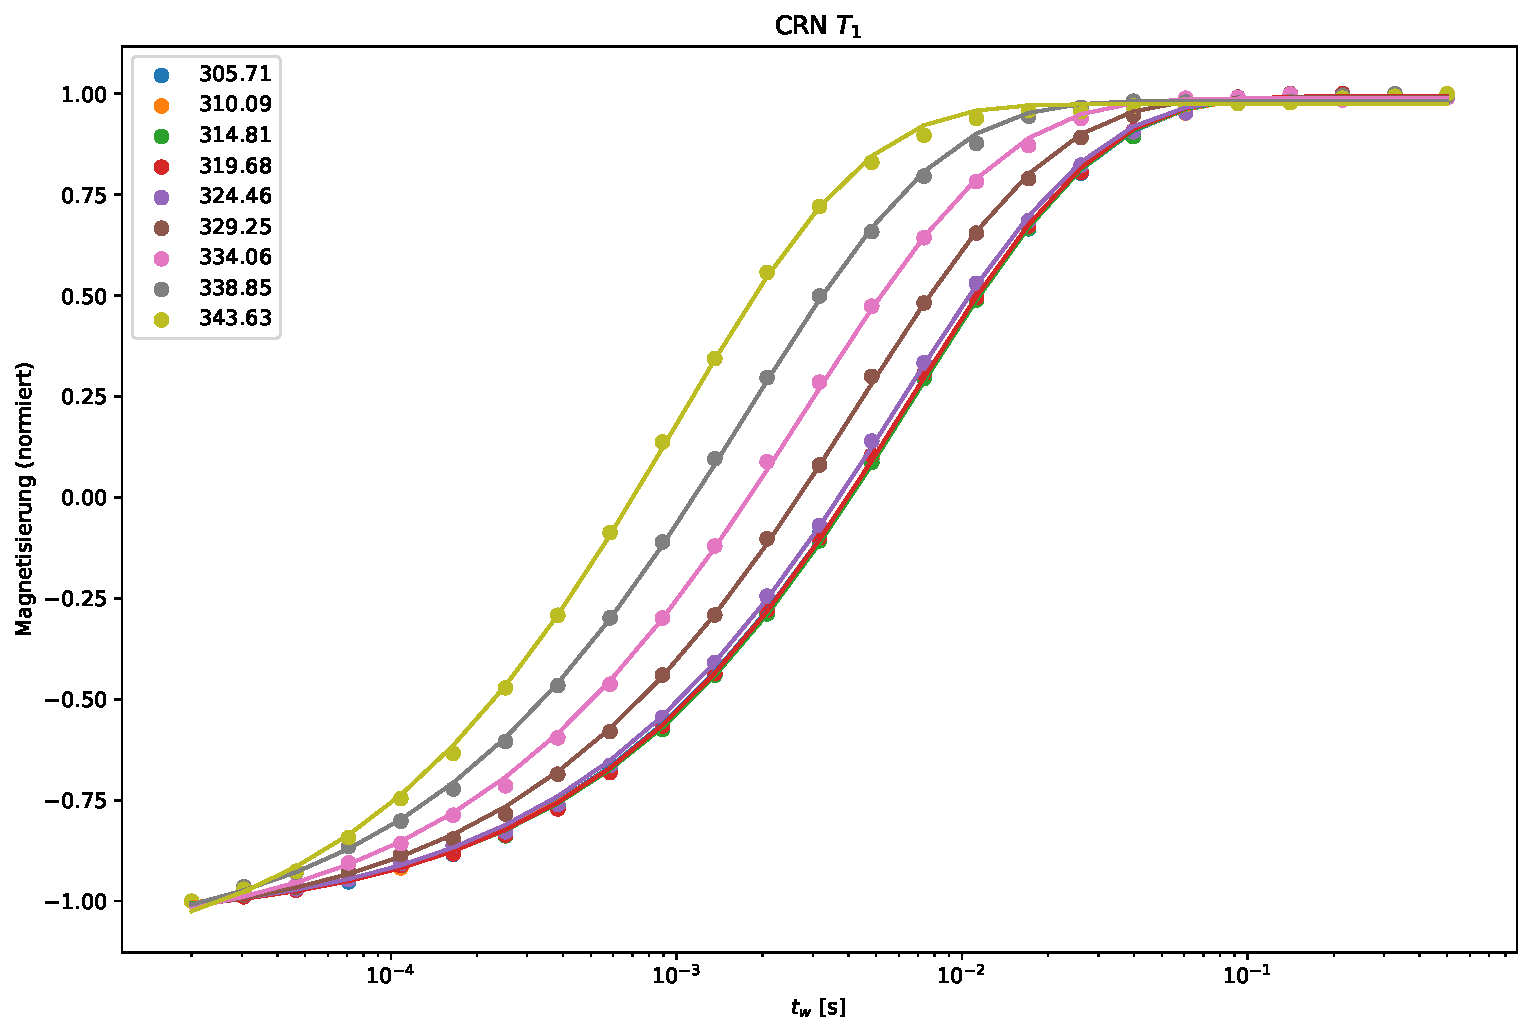
\includegraphics[width=\textwidth]{graphics/plots/T1/t1_roh.pdf}
	\end{center}
	\caption{$T_1$ Rohdaten} \label{fig:res:T_1_roh}
\end{figure}
Während sich die Kurven zwischen $\SI{305}{\kelvin}$ und $\SI{325}{\kelvin}$ sehr ähneln, verschieben sich die Kurven und damit auch die $T_1$-Werte bei höheren Temperaturen zu kürzeren Zeiten.

Dies lässt sich auch in der Gesamtübersicht aller aufgenommenen $T_1$-Daten in Abbildung \ref{fig:res:T_1} erkennen. Während die $T_1$-Zeiten bei Temperaturen von $\SI{250}{\kelvin}$ bis $\SI{325}{\kelvin}$ nahezu unverändert im unteren Millisekunden-Bereich liegen, verkürzen sie sich bei steigenden Temperaturen bis in den zweistelligen Mikrosekunden-Bereich. Es ist ein $T_1$-Minimum bei etwa $\SI{390}{\kelvin}$ auszumachen, ehe die $T_1$-Zeiten stagnieren oder sogar länger werden.

Während die Unsicherheiten weitestgehend vernachlässigbar sind, sind starke Schwankungen über $\SI{390}{\kelvin}$ zu erkennen. Die dort aufgenommenen Daten kann nicht mehr Bedeutung als einer groben Idee der Tatsachen zugemessen werden.

Abgesehen von dem erwähnten Temperaturbereich ist eine gute Übereinstimmung zu den $T_1$-Daten von Zürn \cite{zuern_paper} und zwischen Messungen mit überlappenden Temperaturbereichen zu erkennen, was darauf schließen lässt, dass diese Daten gut reproduzierbar sind. Die am Bruker-Spektrometer aufgenommenen Daten folgen dem gleichen Verlauf und zeigen bis auf den Temperaturbereich zwischen $\SI{360}{\kelvin}$ und $\SI{390}{\kelvin}$ keinen nennenswerte Differenzen; dort aber sind die gemessenen $T_1$-Daten zu leicht längeren Zeiten verschoben.

\begin{figure}
	\begin{center}
		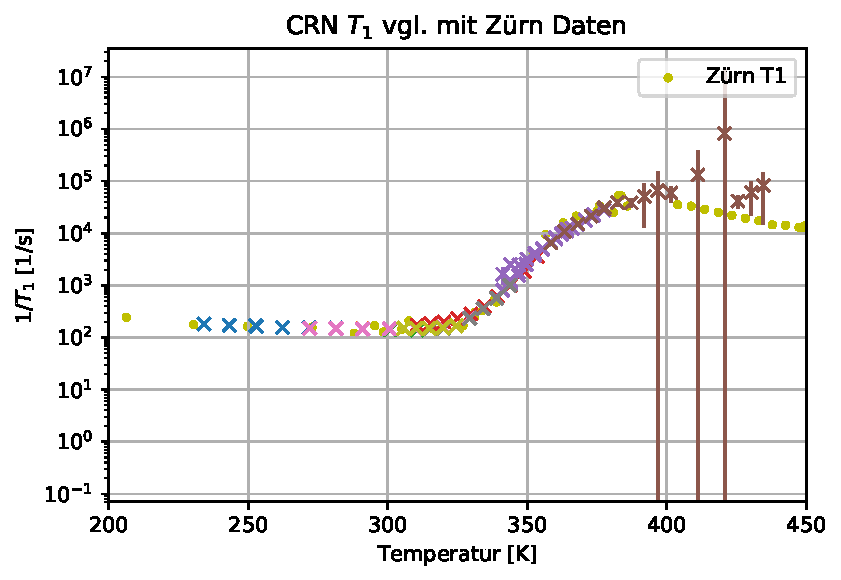
\includegraphics[width=\textwidth]{graphics/plots/T1/t1.pdf}
	\end{center}
	\caption{$T_1$ aus Fits nach Gleichung \eqref{eqn:theo:T_1_fit}. Unterschiedliche Farben indizieren hierbei gesonderte Messreihen; gelbe Punkte bieten einen Vergleich mit Daten von Zürn.} \label{fig:res:T_1}
\end{figure}

\begin{figure}
	\begin{center}
		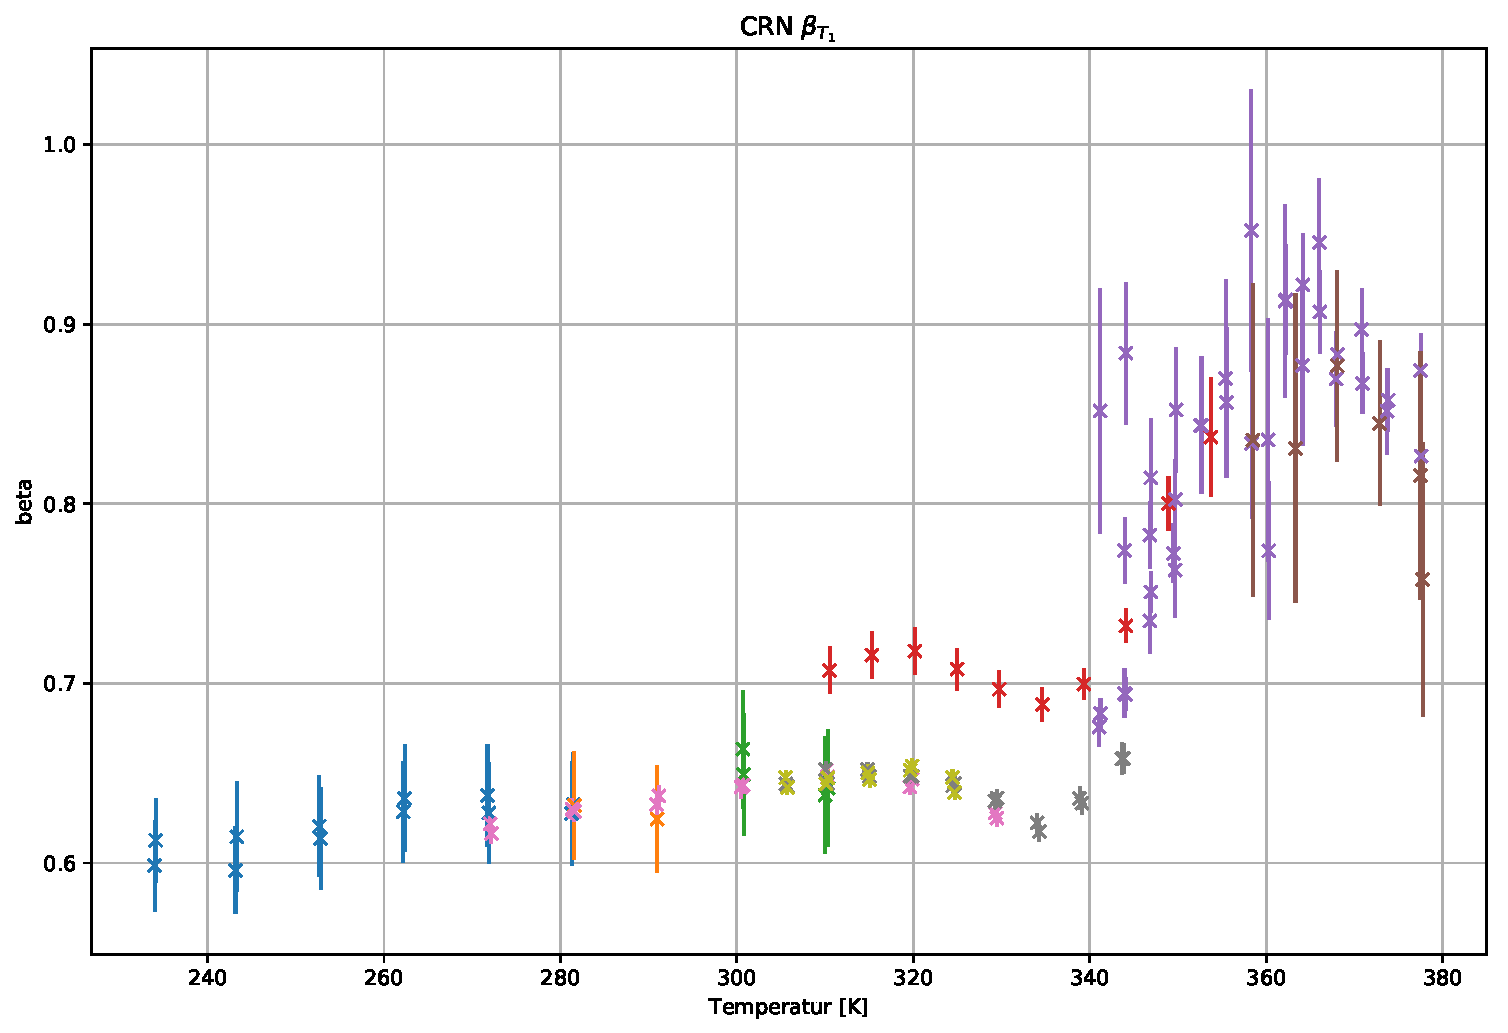
\includegraphics[width=\textwidth]{graphics/plots/T1/t1_beta.pdf}
	\end{center}
	\caption{$\beta_{T_1}$} \label{fig:res:beta_T_1}
\end{figure}


Im oberen Teil der Abbildung \ref{fig:res:T_1} sind die entsprechenden $\beta$ der Fits zu sehen. Von einem Wert von $\SI{0.6}{}$ bei tieferen Temperaturen steigen sie zu einem Wert von etwa $\SI{0.9}{}$ bei Temperaturen über $\SI{350}{\kelvin}$. Dies entspricht etwa den Ergebnissen von Zürn.

Abweichungen gibt es lediglich bei den höheren Temperaturen, wo ein $\beta$ laut \cite{zuern_paper} nahe $\SI{1.0}{}$ liegt, allerdings mit größeren Messunsicherheiten, welche auch hier bei Temperaturen über $\SI{350}{\kelvin}$ zu beobachten sind. Werte über $\SI{380}{\kelvin}$ wurden ausgelassen, da die Messunsicherheiten zu groß waren, als dass den Werten eine Aussage zugestanden werden könnte. Diese stammen daher, dass mit den verwendeten Apparaturen nicht verlässlich Datenpunkte vor $\SI{10}{\micro s}$ aufgenommen werden können. Wenn die $T_1$ Zeit aber in der gleichen Größenordnung liegt und zum Zeitpunkt des $T_1$-Werts das Signal auf etwa $1/e$ abgefallen ist, ist es verständlich, dass ein Fit Schwierigkeiten bereiten kann. Lösen ließe sich dies theoretisch mit einer längeren Evolutionszeit des verwendeten Echos, dies ist aufgrund der kurzen $T_1$- und $T_2$-Zeiten in diesem Temperaturbereich jedoch nicht möglich -- das entstehende Signal ist zu klein um effektiv vom Rauschen getrennt zu werden.

Dennoch ist auffällig, dass trotz der Unsicherheiten von $\beta$ eine relativ gute Übereinstimmung mit den Daten von Zürn vorliegt -- auch von zwei Messreihen zwischen $\SI{315}{\kelvin}$ und $\SI{340}{\kelvin}$ produzierte $\beta$ mit einer Differenz von etwa $\SI{0.1}{}$, sind die entsprechenden $T_1$ in Übereinstimmung miteinander und mit der Literatur. Insofern ist fraglich, welche Aussagekraft den exakten Werten von $\beta$ zugemessen werden kann.

Die Unsicherheiten der mit dem Bruker-Spektrometer bestimmten $\beta$ ist vergleichsweise gering. Dies ist mit der höheren Qualität der Daten (besonders auch in Abbildung \ref{fig:res:bruker_linienform} zu erkennen) und den niedrigeren $T_1$-Werten zu erklären.


\begin{figure}
	\begin{center}
		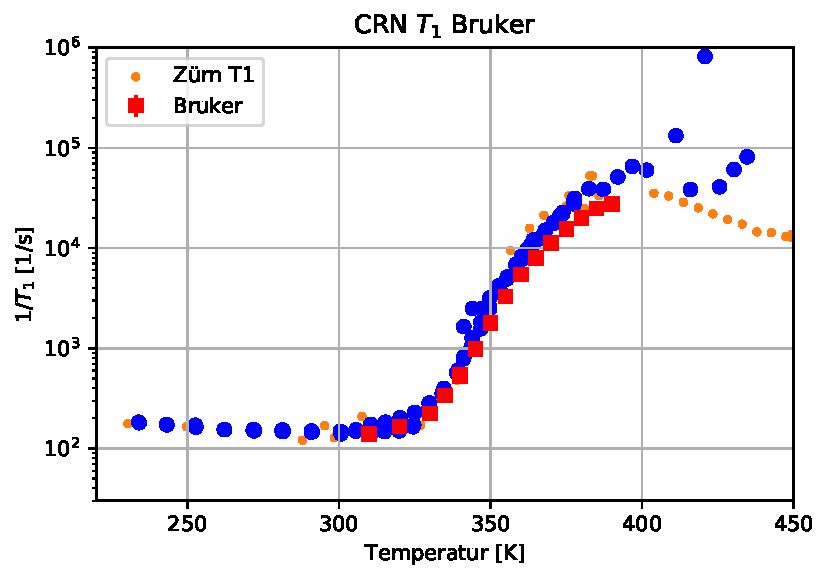
\includegraphics[width=\textwidth]{graphics/plots/BRUKER/bruker_t1.pdf}
	\end{center}
	\caption{Bruker $T_1$} \label{fig:res:bruker_t1}
\end{figure}
Die $T_1$-Werte und die dazugehörigen $\beta$ zeigen gute Übereinstimmung zu den anderen Daten auf.
\begin{figure}
	\begin{center}
		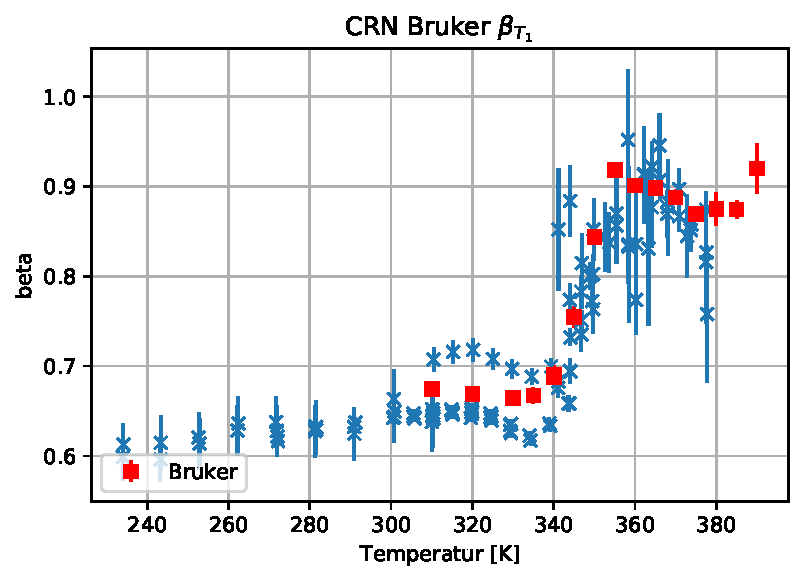
\includegraphics[width=\textwidth]{graphics/plots/BRUKER/bruker_t1beta.pdf}
	\end{center}
	\caption{Bruker $\beta{T_1}$} \label{fig:res:bruker_beta_t1}
\end{figure}



\section{$T_2$} \label{section:res:T_2}

Ähnlich wie $T_1$ ist auch $T_2$ eine wichtige Größe, die Parameter für folgende Messungen bestimmen, oder Aufschluss über Dynamiken geben kann. Die praktikablen Längen von Echos werden von $T_2$ begrenzt. ***

In Abbildung \ref{fig:res:T_2_roh} sind exemplarisch Rohdaten verschiedener Temperaturen zu sehen. Diese wurden mit einem Hahn-Echo mit $\tau = \SI{15}{\micro s}$ aufgenommen und auf den Bereich zwischen $\SI{0}{}$ und $\SI{1}{}$ normiert.

Bruker *** 

\begin{figure}
	\begin{center}
		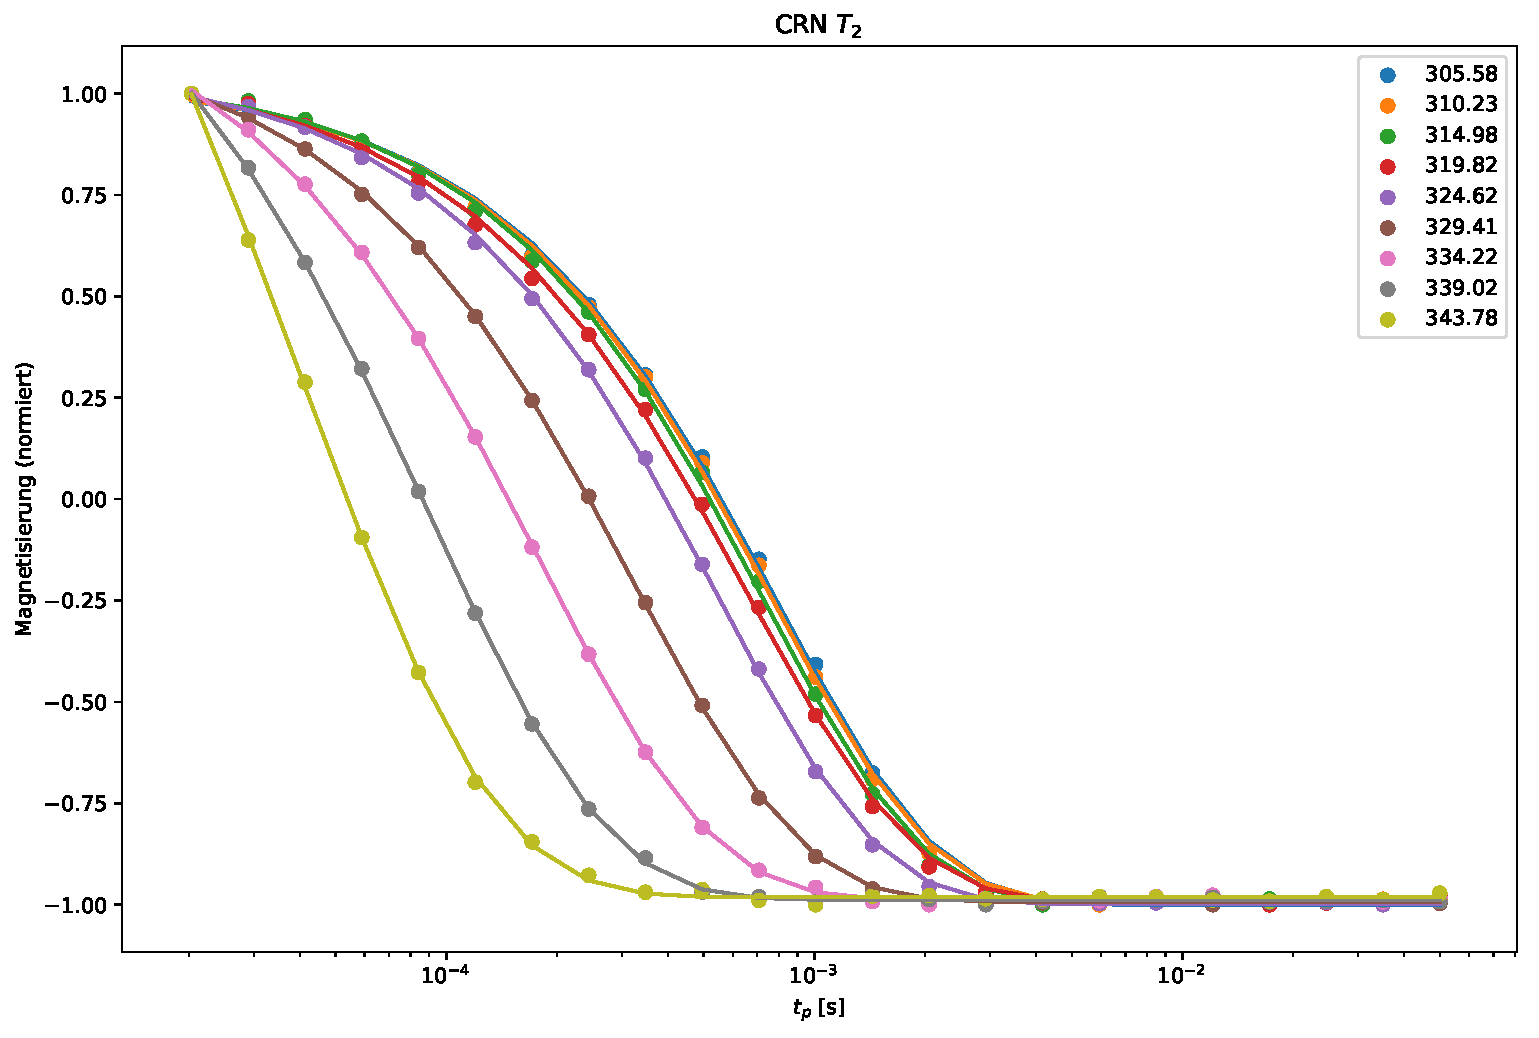
\includegraphics[width=\textwidth]{graphics/plots/T2/t2_roh.pdf}
	\end{center}
	\caption{$T_2$ Rohdaten} \label{fig:res:T_2_roh}
\end{figure}

An diese wurden Fit-Funktionen nach \eqref{eqn:theo:T_2_fit} angelegt, welche als Linien dargestellt sind. Es lässt sich mit den Fits eine gute Übereinstimmung zu den Daten erzielen. Auch hier lässt sich erkennen, dass $T_2$ bei Temperaturen bis etwa $\SI{320}{\kelvin}$ nahezu konstant verbleibt, und zu hoheren Temperaturen kleiner wird.

Abbildung \label{fig:res:T_2} zeigt eine Übersicht über die aufgenommen $T_2$-Werte mit den zugehörigen $\beta$ der Fits. Unter $\SI{320}{\kelvin}$ verbleiben erstere im niedrigen Millisekunden-Bereich, ehe sie deutlich kürzer werden und sich bei etwa $\SI{360}{\kelvin}$ ein Minimum zeigt. Die Werte des Bruker-Spektrometers sind hiermit in guter Übereinstimmung, wobei wiederum festzuhalten ist, dass die Messunsicherheiten geringer sind. Ein zweites Minimum zeigt sich bei etwa $\SI{400}{\kelvin}$, das, ebenso wie das erste, im zweistelligen Mikrosekunden-Bereich liegt. Zwischen $\SI{400}{\kelvin}$ und $\SI{410}{\kelvin}$ ist zu erkennen, dass -- wohl durch die Kürze von $T_2$ bei diesen Temperaturen -- deutlich größere Unsicherheiten als im Rest der Messreihe vorliegen, wo sie in guter Näherung vernachlässigbar sind. 

Auch die $\beta$-Werte zeigen bei höheren Temperaturen deutlich größere Unsicherheiten, hier allerdings schon zwischen $\SI{390}{\kelvin}$ und $\SI{425}{\kelvin}$, was eine Bestimmung der Werte verkompliziert. Sie scheinen zwischen $\SI{1}{}$ und $\SI{2}{}$ zu liegen. Bei tieferen Temperaturen klärt sich das Bild etwas: Während die Daten des OBI-Spektrometers ein $\beta$ zwischen $\SI{1}{}$ und $\SI{1.5}{}$ bei Temperaturen bis $\SI{350}{\kelvin}$ suggerieren, zeigen die Daten des Bruker-Spektrometers ein $\beta$ um $\SI{1}{}$ -- mit geringerer Unsicherheit. Bei nochmals tieferen Temperaturen scheint $\beta$ konsistent bei rund $\SI{1}{}$ zu liegen.

\begin{figure}
	\begin{center}
		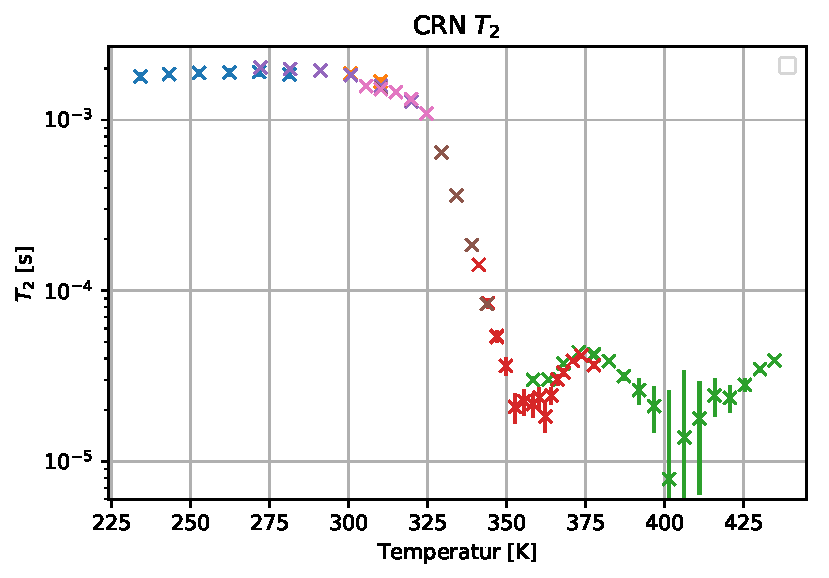
\includegraphics[width=\textwidth]{graphics/plots/T2/t2.pdf}
	\end{center}
	\caption{$T_2$ gegen Temperatur} \label{fig:res:T_2}
\end{figure}

\begin{figure}
	\begin{center}
		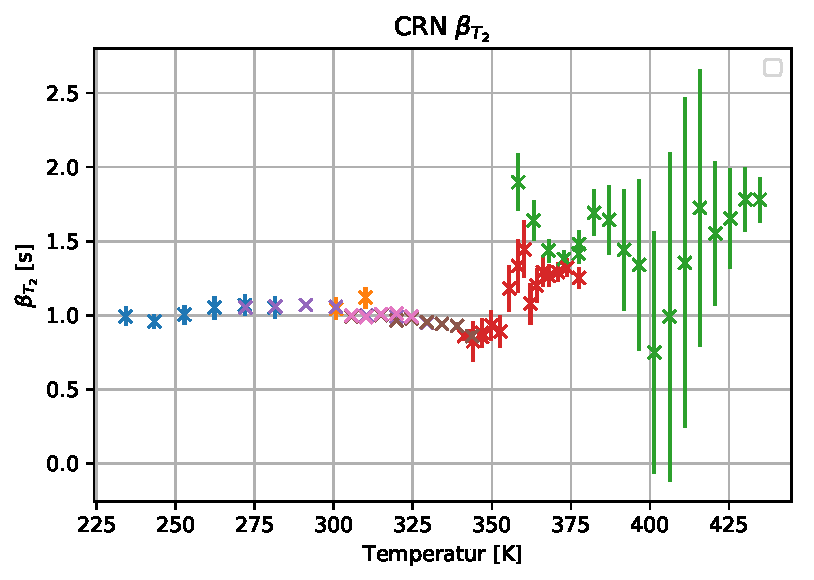
\includegraphics[width=\textwidth]{graphics/plots/T2/t2_beta.pdf}
	\end{center}
	\caption{$\beta_{T_2}$ gegen Temperatur} \label{fig:res:beta_T_2}
\end{figure}

\begin{figure}
	\begin{center}
		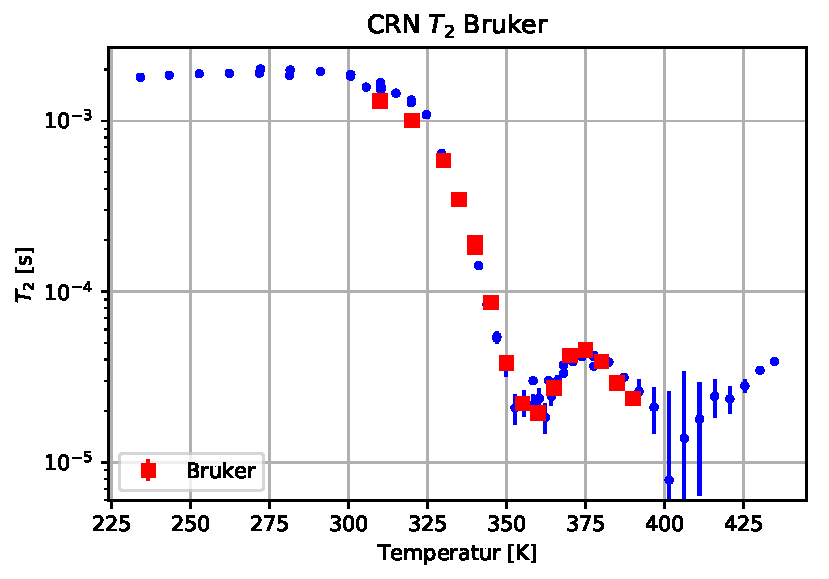
\includegraphics[width=\textwidth]{graphics/plots/BRUKER/bruker_t2.pdf}
	\end{center}
	\caption{Bruker $T_2$} \label{fig:res:bruker_t2}
\end{figure}

\begin{figure}
	\begin{center}
		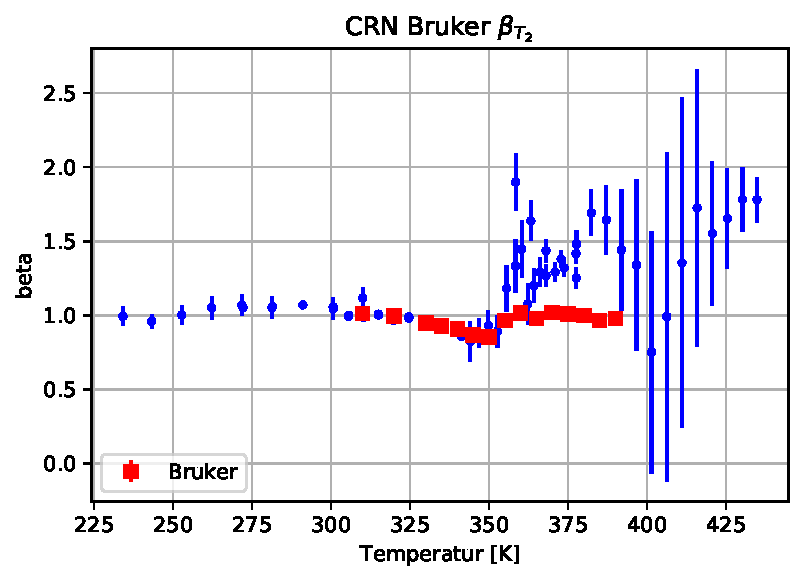
\includegraphics[width=\textwidth]{graphics/plots/BRUKER/bruker_t2beta.pdf}
	\end{center}
	\caption{Bruker $\beta{T_2}$} \label{fig:res:bruker_beta_t2}
\end{figure}




\section{$F_2$} \label{section:res:F_2}

Mit der Absicht einen möglichen Betaprozess zu identifizieren, wurden $F_2$-Messungen, also stimulierte Echos, durchgeführt. Dazu wurden am Spektrometer OBI über eine Reihe von Temperaturen von $\SI{230}{\kelvin}$ bis $\SI{310}{\kelvin}$ und Evolutionszeiten von $\SI{50}{\micro s}$ bis $\SI{1000}{\micro s}$ Messungen durchgeführt. Es wurde eine Drei-Puls-Folge verwendet und sowohl C ***

Die meisten ähnelten der hier beispielhaft ausgewählten Messung bei $\SI{280}{\kelvin}$ und einer Evolutionszeit von $t_p = \SI{1000}{\micro s}$: Die Daten lassen sich schwerlich oder gar nicht von einer $T_1$-Kurve unterscheiden, die bei gleicher Temperatur aufgenommen wurde, wie in Abbildung \ref{fig:res:F_2_tieftemp} zu sehen. Es scheint daher nicht möglich, in diesem Temperaturbereich mit dieser Methode Aussagen über mögliche Dynamik treffen zu können.
\begin{figure}
	\begin{center}
		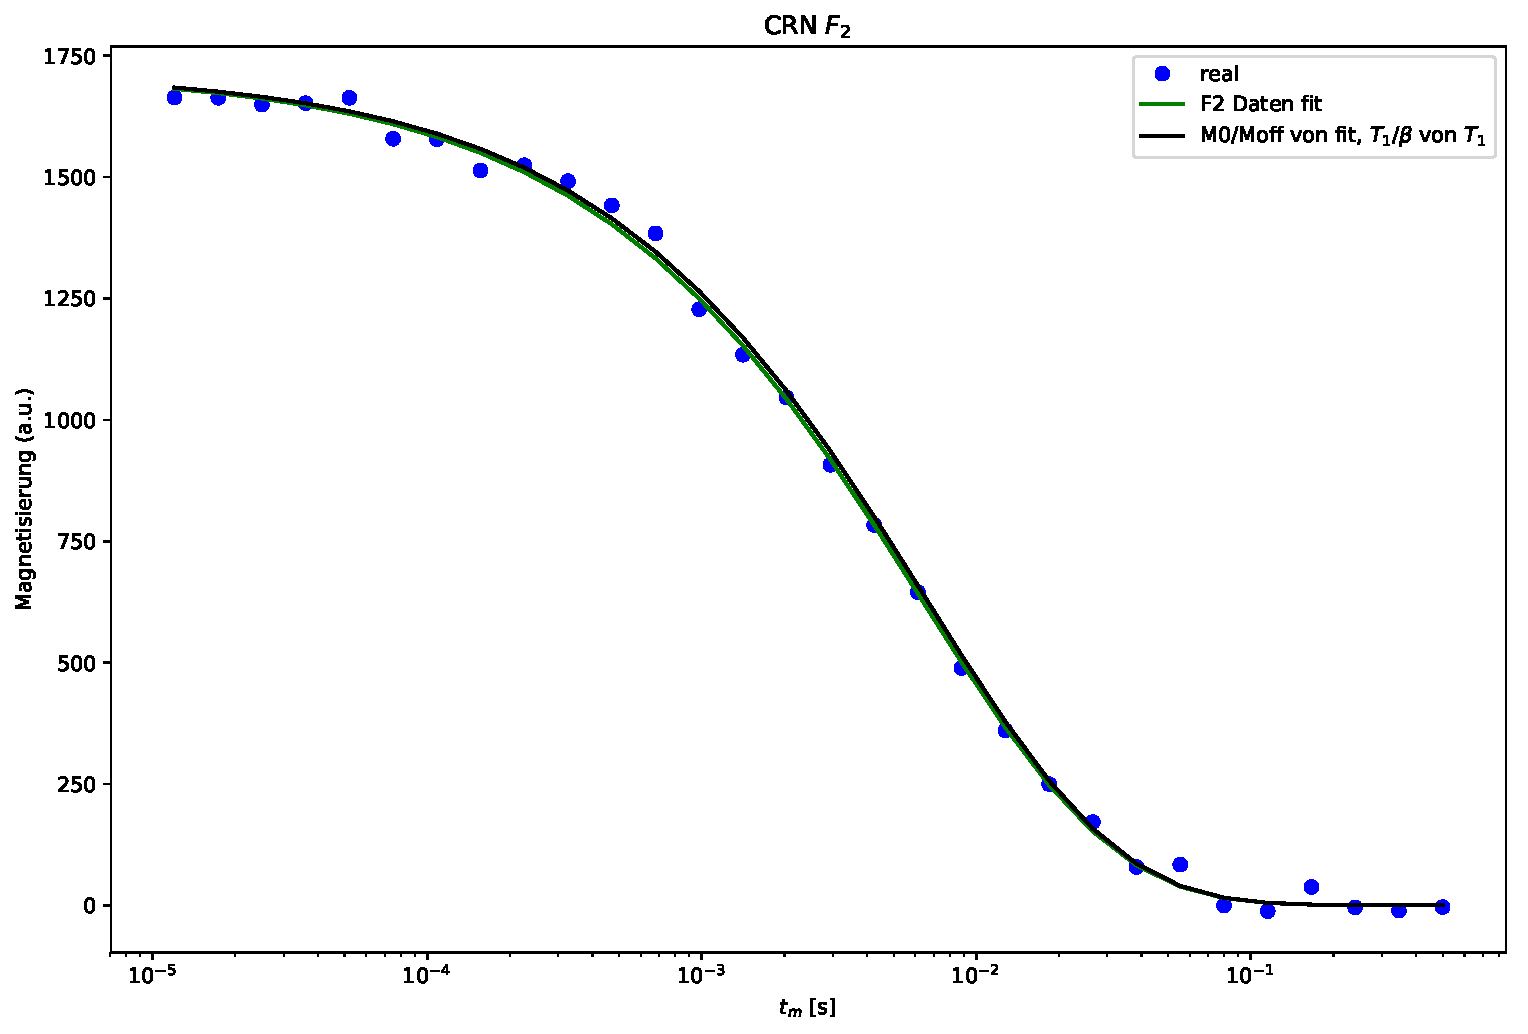
\includegraphics[width=\textwidth]{graphics/plots/F2/f2_tieftemp.pdf}
	\end{center}
	\caption{$F_2$ bei tiefen Temperaturen} \label{fig:res:F_2_tieftemp}
\end{figure}

Lediglich bei den Temperaturen $\SI{300}{\kelvin}$ und $\SI{310}{\kelvin}$, sowie $t_p = \SI{1000}{\micro s}$ konnte ein nennenswerter Unterschied zu reinen $T_1$-Kurven beobachtet werden; die entsprechenden Messungen sollen im Folgenden besprochen werden.

Einen Fit der Form *** (Formel) direkt an die Messwerte anzulegen erwies sich als schwierig, daher wurde folgende Schritte für eine Auswertung durchgeführt: An die Daten wurde folgende Funktion gefittet:
\begin{align}
	M_{F_2} (t_m) = M_0 \left[ \exp{ \left(- { \left( \frac{t_m}{F_2} \right) }^{\beta_{F_2}} \right)} \right] + M_\text{off} \label{eqn:res:F_2_fit}
\end{align}
Dieser Fit stellt die grüne Kurve in Abbildung \ref{fig:res:F_2_fit} dar.
\begin{figure}
	\begin{center}
		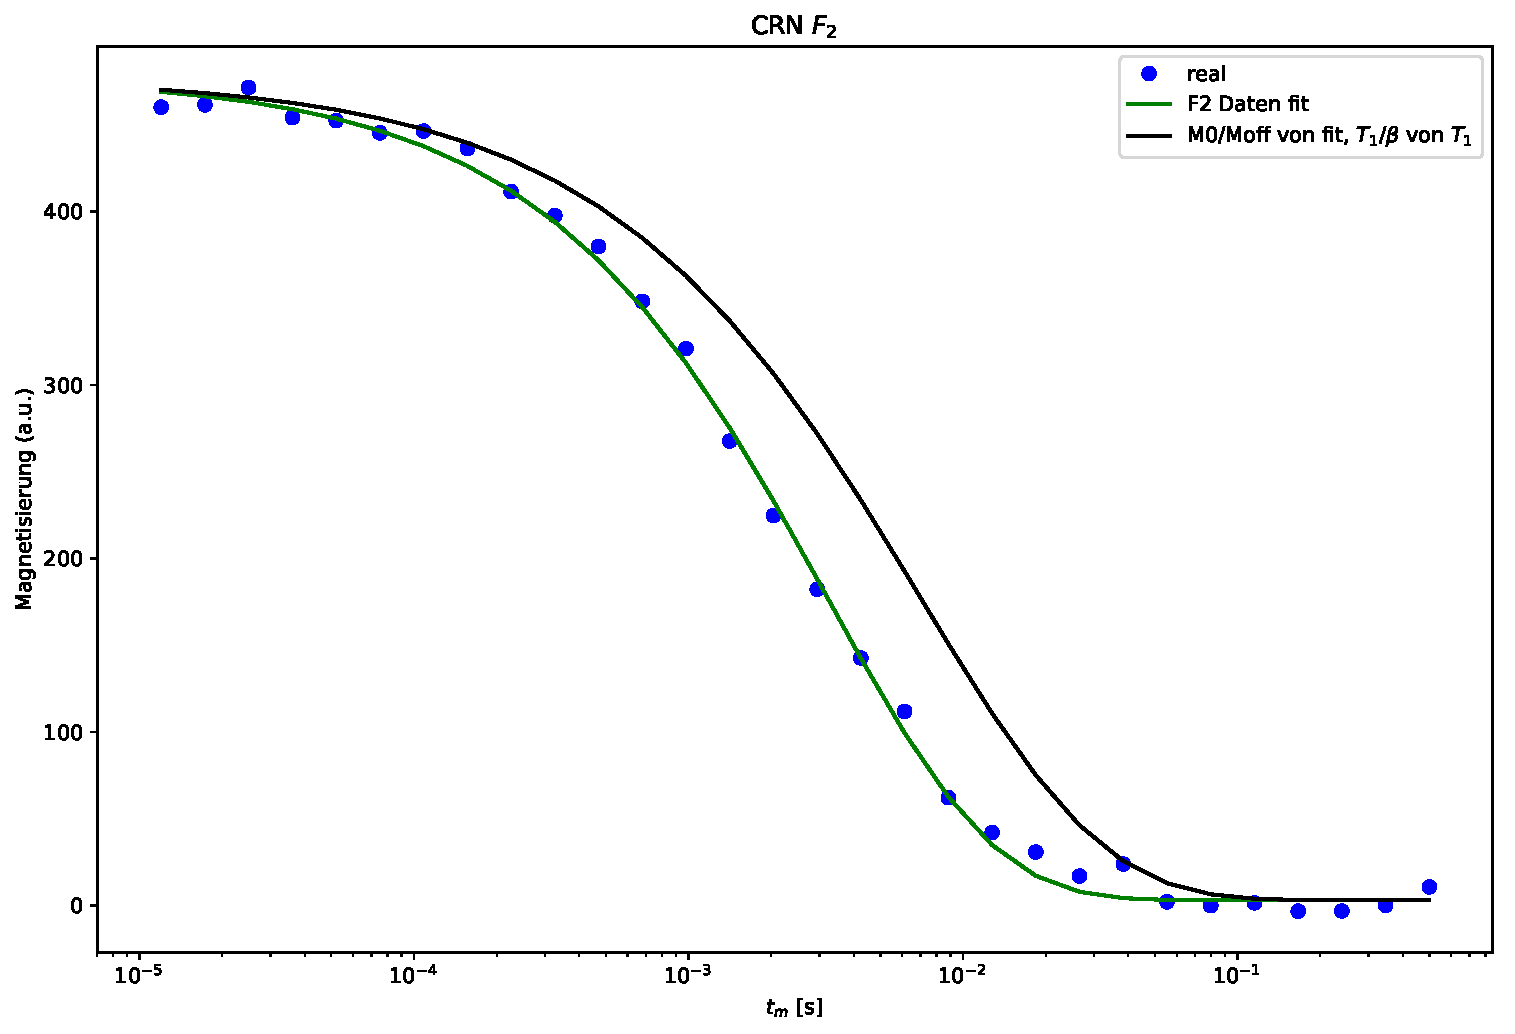
\includegraphics[width=\textwidth]{graphics/plots/F2/f2_fits.pdf}
	\end{center}
	\caption{$F_2$ Fits} \label{fig:res:F_2_fit}
\end{figure}
Die Werte $F_2$ und $\beta_{F_2}$ wurden dann durch $T_1$ und $\beta_{T_1}$ einer $T_1$-Messung gleicher Temperatur ersetzt -- das Resultat ist als schwarze Kurve gezeigt. Dieses Vorgehen macht es möglich, die $T_1$-Kurve an die $F_2$-Daten anzupassen. Es wurden nun die Daten durch die angepasste $T_1$-Kurve um den entsprechenden Anteil zu eliminieren. Das Resultat ist in Abbildung \ref{fig:res:F_2_T_1} gezeigt.
\begin{figure}
	\begin{center}
		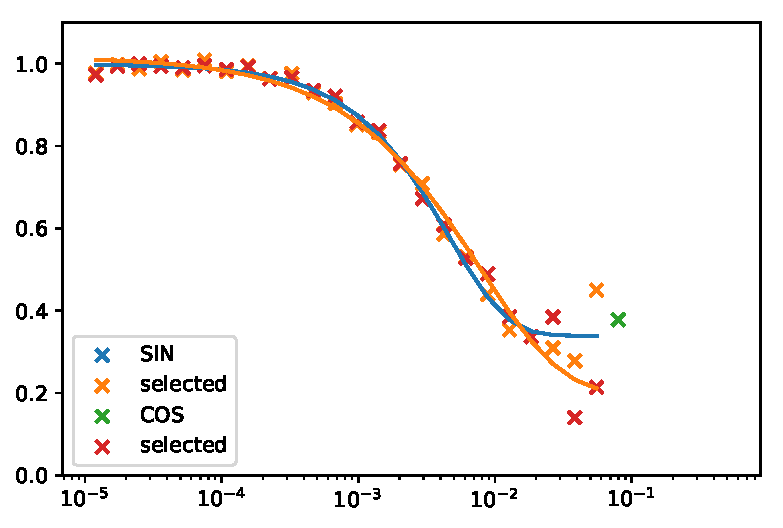
\includegraphics[width=\textwidth]{graphics/plots/F2/f2_fit.pdf}
	\end{center}
	\caption{$F_2$ geteilt durch Fit, 310K} \label{fig:res:F_2_T_1}
\end{figure}
Da die Daten bei Mischzeiten von über Eine ähnliche Auswertung wurde durchgeführt, wobei anstatt der Halbwertsbreite die Amplitude bei einer bestimmten Frequenz (beispielsweise )
 stark streuen wurden sie nicht dargestellt. An verbleibenden Punkte wiederum kann ein Kohlrausch-Fit angelegt werden, um über den beschriebenen Umweg zu einer Funktion ähnlich der aus Formel *** zu gelangen.

Es wurden je zwei Messungen einer Cos-Cos-Pulsfolge und einer Sin-Sin-Pulsfolge bei $\SI{310}{\kelvin}$ durchgeführt, sowie je eine Messung bei $\SI{300}{\kelvin}$. Die Resultate finden sich in Tabelle \ref{tab:res:F_2}

\begin{table}[H]
	\centering
	\begin{tabular}{lllll}
		\hline
		Temperatur & Sin-Sin $\tau$ & Sin-Sin $\beta$ & Cos-Cos $\tau$ & Cos-Cos $\beta$ \\ \hline
		$\SI{300}{\kelvin}$ (Lauf 1) & $\SI{5.26 (94)}{\milli s}$ & $\SI{0.95 (18)}{}$ & $\SI{3.68 (63)}{\milli s}$ & $\SI{1.30 (34)}{}$ \\
		$\SI{310}{\kelvin}$ (Lauf 1) & $\SI{3.27 (122)}{\milli s}$ & $\SI{1.12 (56)}{}$ & $\SI{9.95 (432)}{\milli s}$ & $\SI{0.74 (21)}{}$ \\
		$\SI{310}{\kelvin}$ (Lauf 2) & $\SI{4.23 (37)}{\milli s}$ & $\SI{1.01 (10)}{}$ & $\SI{3.28 (7)}{\milli s}$ & $\SI{0.71 (1)}{}$ \\
		 \hline
	\end{tabular}
	\caption{Resultate der $F_2$-Messungen. Sin-Sin und Cos-Cos beziehen sich auf die jeweils verwendete Pulsfolge, $\tau$ und $\beta$ sind die mit den Fits bestimmten Parameter der Zeitkonstante und der Streckung der Exponentialfunktion. \label{tab:res:F_2}}
\end{table}

Es ist zu erkennen, dass die Größen zwischen den zwei Durchläufen teils mehr schwanken als zwischen zwei Temperaturen oder im Vergleich zwischen Sin-Sin- und Cos-Cos-Pulsfolgen. Da die Unsicherheiten zudem in Fällen beinahe $\SI{50}{\percent}$ erreicht, müssen diese Ergebnisse mit Vorsicht genossen werden. Es ist aber klar, dass sich die Zeitkonstanten nicht in einem Bereich befinden, wo sie für einen Betaprozess nach den Überlegungen zu erwarten wären. ***



\section{Spektren Dynamik} \label{section:res:spekdyn}

Eine weitere Untersuchung zu möglicher Dynamik wurde an der sich ändernden Linienform von pulslängenabhängigen Spektren durchgeführt. Die Details von CRN-Spektren sollen in einem späteren Abschnitt diskutiert werden.

Es wurde beobachtet, dass Spektren die mit einem Hahn-Echo mit unterschiedlicher Evolutionszeit aufgenommen wurden, eine unterschiedliche Linienform zeigen. Die Halbwertsbreiten der normierten Spektren ist also evolutionszeitabhängig, und das bei verschiedenen Temperaturen in verschiedenen Maßen. Dies lässt sich in Abbildung \ref{fig:res:spekdyn_305K} im Vergleich mit Abbildung \ref{fig:res:spekdyn_325K} erkennen, wo pulslängenabhängige Spektren für die Temperaturen $\SI{305}{\kelvin}$ bzw. $\SI{325}{\kelvin}$ gezeigt sind.
\begin{figure}
	\begin{center}
		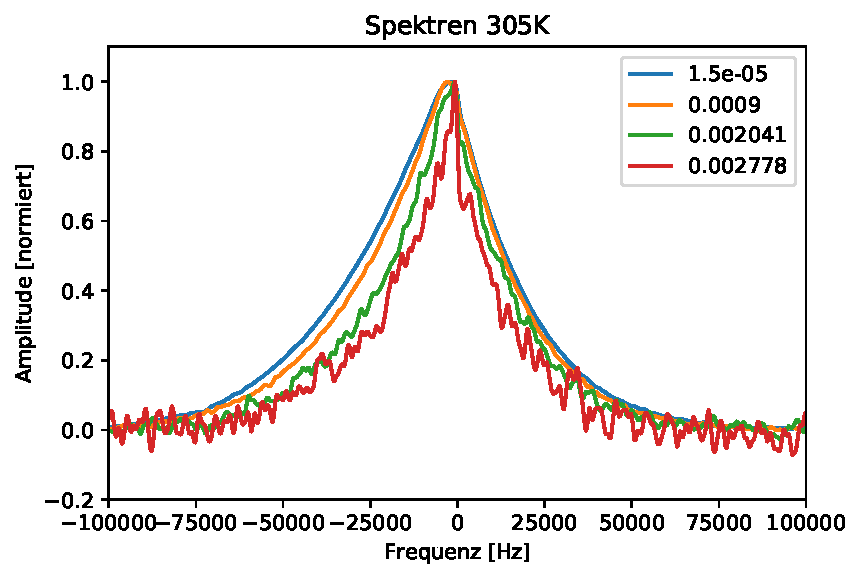
\includegraphics[width=\textwidth]{graphics/plots/SPEKDYN/spekdyn_305K.pdf}
	\end{center}
	\caption{Spektren Linienform($\tau$) 305K} \label{fig:res:spekdyn_305K}
\end{figure}
\begin{figure}
	\begin{center}
		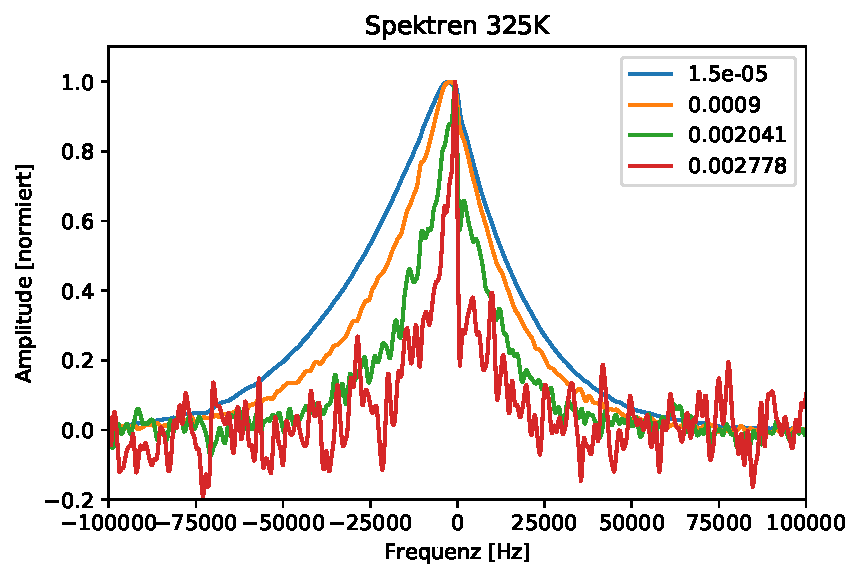
\includegraphics[width=\textwidth]{graphics/plots/SPEKDYN/spekdyn_325K.pdf}
	\end{center}
	\caption{Spektren Linienform($\tau$) 325K} \label{fig:res:spekdyn_325K}
\end{figure}
Alle Spektren wurden mit dem OBI-Spektrometer aufgenommen; dabei wurde ein Hahn-Echo mit variabler Evolutionszeit verwendet und die Spektren mit $\SI{500}{Hz}$ apodisiert.

Zur Untersuchung dieses Phänomens wurde für jede Temperatur die Halbwertsbreite gegen die Evolutionszeit $t_p$ aufgetragen. Da die Spektren bei hohen Pulslängen teils sehr verrauscht sind, wurden die aufgetragengen Evolutionszeiten auf $\SI{2}{\milli s}$ begrenzt. Da diese Daten wurden Kohlrausch-Fits angelegt, die, zusammen mit dem Daten, als durchgezogene Linien in Abbildung \ref{fig:res:spekdyn_fits} zu sehen sind.
\begin{figure}
	\begin{center}
		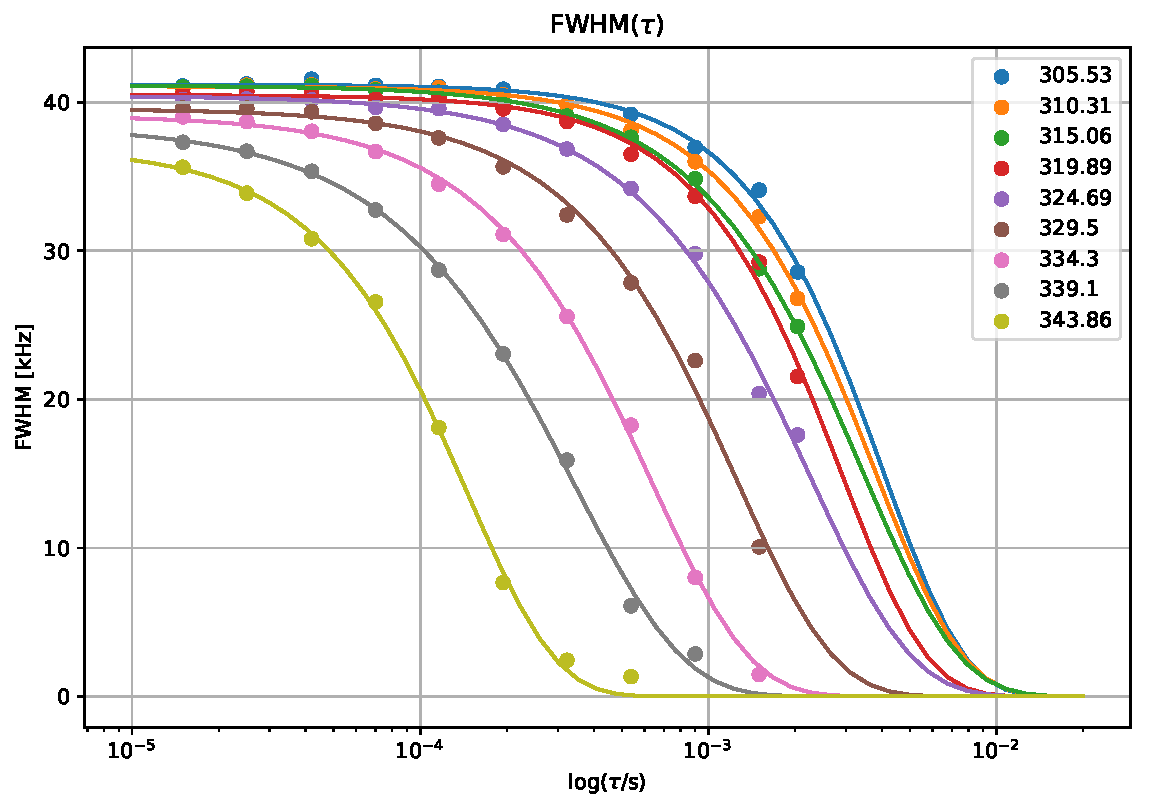
\includegraphics[width=\textwidth]{graphics/plots/SPEKDYN/spekdyn_fits.pdf}
	\end{center}
	\caption{FWHM Fits} \label{fig:res:spekdyn_fits}
\end{figure}


Es wurde eine weitere, ähnliche Auswertung wurde durchgeführt, wobei anstatt der Halbwertsbreite die Amplitude bei einer bestimmten Frequenz (beispielsweise bei $\SI{-10}{\kilo Hz}$) als Variable genommen wurde. Die Ergebnisse glichen der der Halbwertsbreiten-Betrachtung, waren aber durchgehend mit größeren Unsicherheiten behaftet. Dies lässt sich durch die stark verrauschten Spektren bei hohen Evolutionszeiten erklären, die zu stark schwankenden Amplituden führen, welche wiederum einen guten Fit der Daten schwierig gestalten.





\section{Spektren} \label{section:res:spektren}

Der zweite Abschnitt dieser Arbeit beschäftigt sich mit der Linienform-Untersuchung an CRN. Bei der Auswertung von Spektren wurde eine ungewöhnlich erscheinende Verbreiterung der Spektren in einem Temperaturbereich beobachtet, wo, aufgrund von Bewegungsverschmälerung, eher kleinere Halbwertsbreiten zu erwarten wären. Zur Untersuchung der Gegebenheiten wurden, neben einer vielzahl von experimenteller Spektren, Computer-Simulationen angefertigt, und versucht eine theoretische Erklärung der Daten zu bieten.

Um eine Übersicht zu schaffen, werden zuerst die Linienformen der Spektren aus den verschiedenen Quellen in Abhängigkeit der Temperatur präsentiert. Abbildung \ref{fig:res:spek_linienform} zeigt die am OBI-Spektrometer aufgenommenen Spektren; die Temperaturen reichen von etwa $\SI{234}{\kelvin}$ bis etwa $\SI{435}{\kelvin}$. Sie wurden mit einem Hahn-Echo mit einer Evolutionszeit von $t_p = \SI{15}{\micro s}$ aufgenommen und mit $\SI{500}{Hz}$ apodisiert. Es wurden je $\SI{8192}{}$ Datenpunkte mit einer Frequenz von $\SI{2}{MHz}$ erstellt. Die Spektren wurden in mehreren Messreihen aufgenommen und stellen eine repräsentative Auswahl dar, die es erlaubt, den Verlauf der Linienform nachzuvollziehen, ohne zu stark an Übersicht zu verlieren.
\begin{figure}
	\begin{center}
		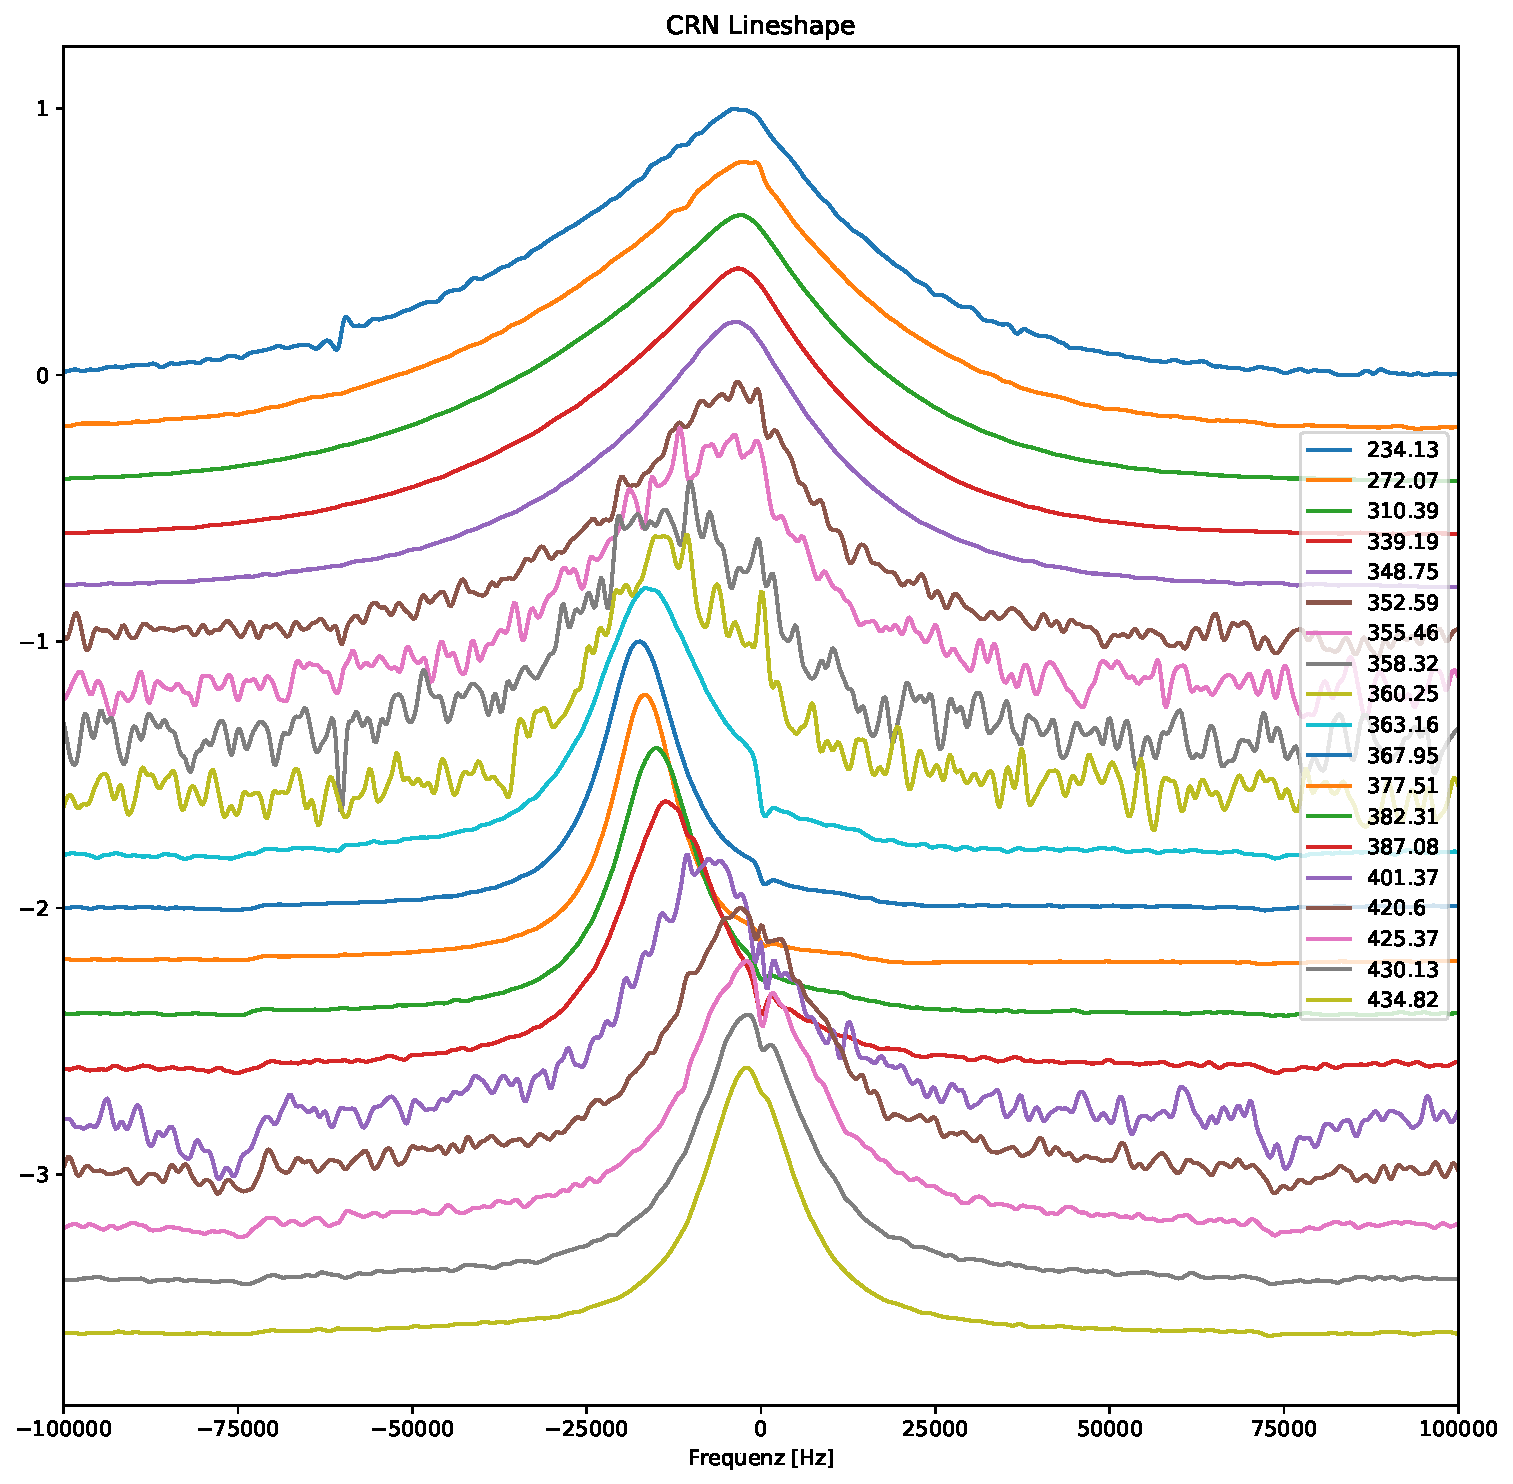
\includegraphics[width=\textwidth]{graphics/plots/SPEK/spek_lineshape.pdf}
	\end{center}
	\caption{Spektren Linienform} \label{fig:res:spek_linienform}
\end{figure}
Bei tiefen Temperaturen ist eine Form zu beobachten, die der des Czjzek-Spektrums aus Kapitel (***) ähnelt. Diese hält sich über weite Temperaturen, von etwa $\SI{235}{\kelvin}$ bis etwa $\SI{350}{\kelvin}$, fast unverändert. Zu höheren Temperaturen ändert sich die Linienform, sie nimmt die einer Lorentz-Funktion an, während die Spektren gleichzeitig schmaler werden und sich der Schwerpunkt zu niedrigeren Frequenzen verschiebt. Diese Bewegung findet ein Ende bei etwa $\SI{367}{\kelvin}$: Zu höheren Temperaturen verbreitern sich die Spektren wieder, ehe sie ab $\SI{410}{\kelvin}$ wieder schmaler werden. Der Schwerpunkt verschiebt sich ab 375K wieder gegen $\SI{0}{Hz}$, wo es ab 400K verweilt. Die Linienform ändert sich nicht mehr.

Es ist auffällig, dass die Qualität der Spektren stark mit der Temperatur schwankt. Zwischen $\SI{235}{\kelvin}$ und $\SI{350}{\kelvin}$, $\SI{363}{\kelvin}$ und $\SI{387}{\kelvin}$, sowie zwischen $\SI{430}{\kelvin}$ und $\SI{435}{\kelvin}$ weisen die Spektren vergleichsweise geringes Rauschen und somit eine glattere Form auf. Das abschnittweise höhere Schwankungen lassen sich durch $T_2$-Minima bei den entsprechenden Temperaturen erklären -- diese sorgen für einen schnellen Abfall des Signals und entsprechend verrauschte Spektren. *** Lorentz

Die am Bruker-Spektrometer aufgenommenen Spektren decken einen Temperaturbereich von $\SI{310}{\kelvin}$ bis $\SI{390}{\kelvin}$ ab, und wurden ebenfalls mit einem Hahn-Echo mit einer Evolutionszeit von $\SI{15}{\micro s}$ erstellt und mit $\SI{500}{Hz}$ apodisiert. Hier wurden je $\SI{4096}{}$ Datenpunkte mit einer Frequenz von $\SI{0.5}{MHz}$ aufgenommen. Da mit diesem Spektrometer weitaus weniger Spektren erstellt wurden als mit dem OBI-Spektrometer können in Abbildung \ref{fig:res:bruker_linienform} alle Spektren präsentiert werden.
\begin{figure}
	\begin{center}
		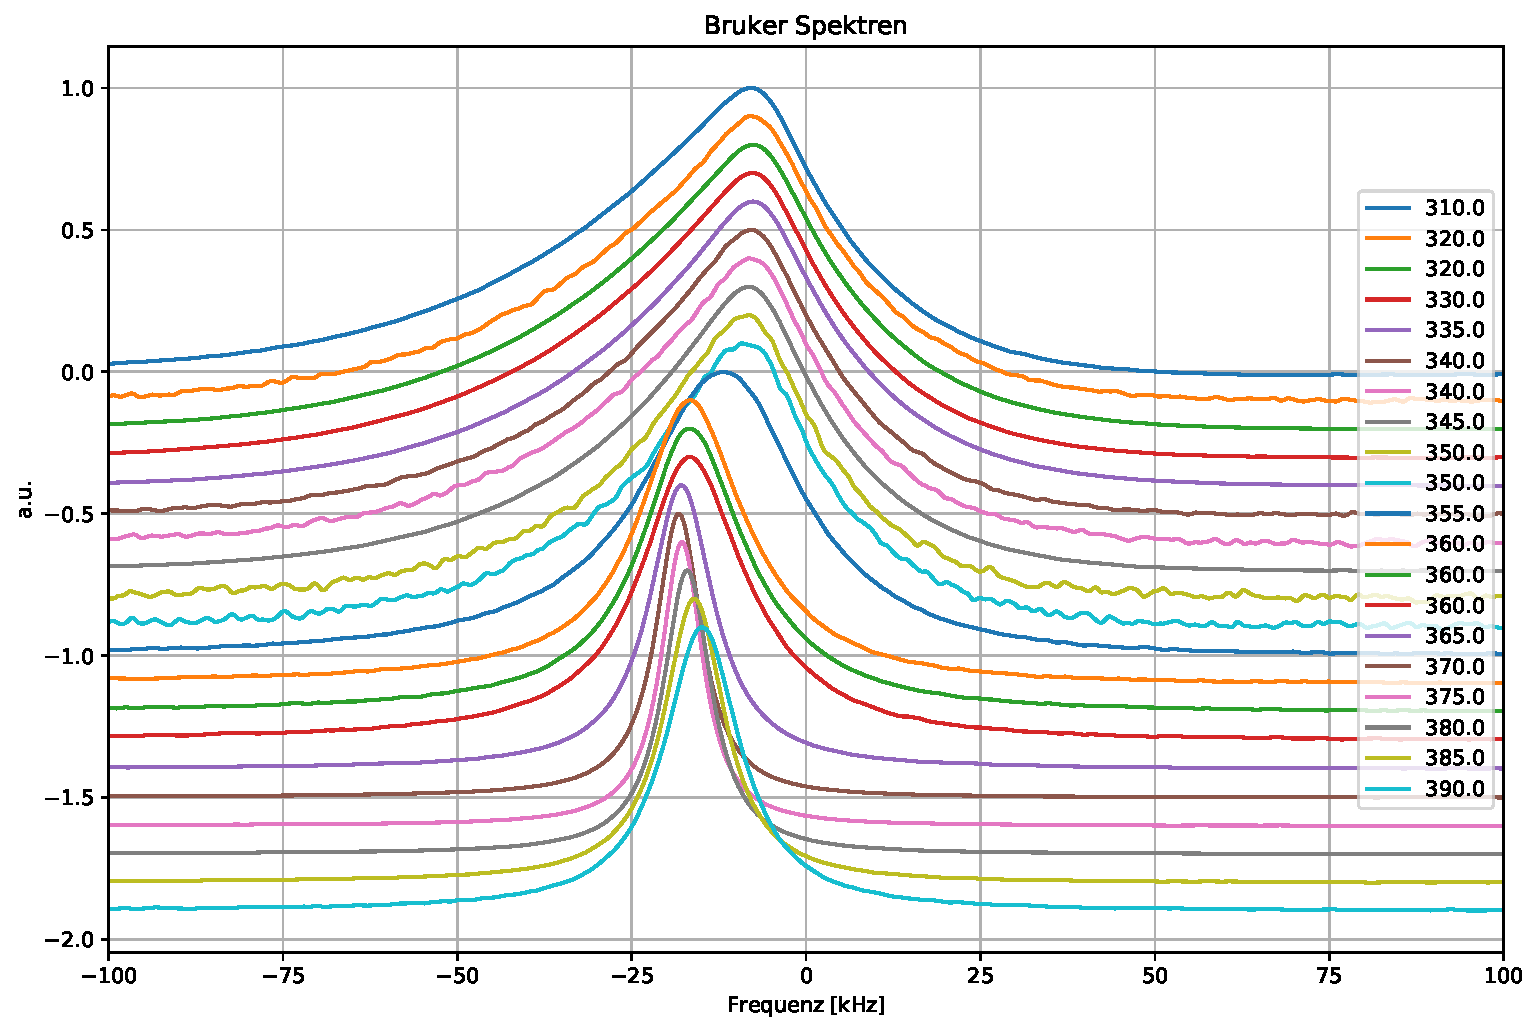
\includegraphics[width=\textwidth]{graphics/plots/BRUKER/bruker_lineshape.pdf}
	\end{center}
	\caption{Bruker Linienform} \label{fig:res:bruker_linienform}
\end{figure}
Der Verlauf der Linienform gleicht den Beschriebenen in dem entsprechenden Temperaturbereich gut. Es ist das geringe Rauschen der Spektren zu beachten, das, wie auch insbesondere die $T_2$-Daten ein Beleg für hohe Datenqualität des Bruker-Spektrometers in diesem Kontext ist.

Als Ergänzung zu den experimentellen Daten wurden simulierte Spektren angefertigt. Dazu wurde die in Kapitel (***) vorgestellte Simulations-Software verwendet. Es wurden FIDs mit $\SI{4096}{}$ Datenpunkten mit einem Abstand von je $\SI{0.5}{\micro s}$, was einer Frequenz von $\SI{0.5}{MHz}$ entspricht, aufgenommen. Um einen Mittelwert zu bilden wurden, je nach Spektrum, zwischen $10^{7}$ und $10^{9}$ einzelne Simulationen gemittelt. Als Modell wurde ein isotroper Zufallssprung gewählt, welcher eine Czjzek-Verteilung als Ausgangspunkt hat; dieses war der simulierten Quadrupol-Wechselwirkung zweiter Ordnung ausgesetzt. Zur Bestimmung der Lebensdauer eines bestimmten Zustandes wird eine Exponentialverteilung genutzt, deren Parameter, die Lebenszeit, eine Verknüpfung mit Temperaturen ermöglicht. Es wurde eine Vogel-Fulcher-Funktion für die Lebenszeit mit den Parametern für CRN aus Kapitel (*** Andere $\tau_c$s, zum Beispiel aus DOI: 10.1103/PhysRevE.81.051504 zeigen keinen großen Unterschied.) verwendet. Die resultierenden Spektren sind in Abbildung \ref{fig:res:sim_linienform} zu sehen.
\begin{figure}
	\begin{center}
		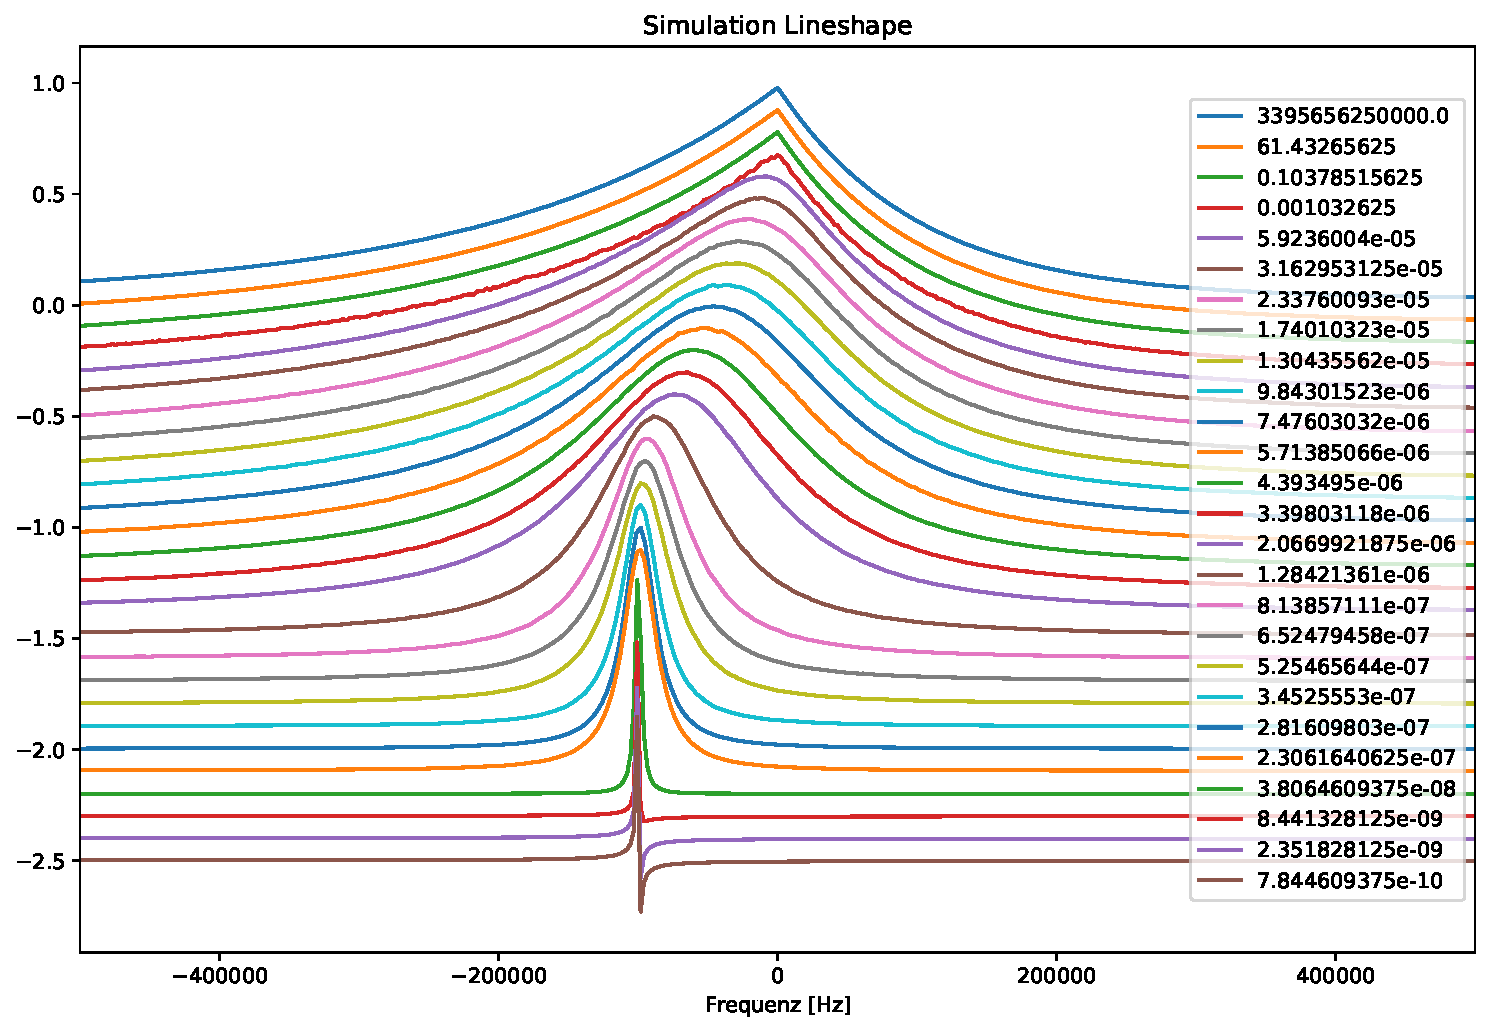
\includegraphics[width=\textwidth]{graphics/plots/SIM/sim_lineshape.pdf}
	\end{center}
	\caption{Simulation Linienform} \label{fig:res:sim_linienform}
\end{figure}
Bei tiefen Temperaturen gleichen die simulierten Spektren den experimentellen sehr. (*** extra Vergleich?) Auch ist der Übergang zur Lorentz-Form, verbunden mit der Verschiebung des Schwerpunkts und Verschmälerung der Spektren bei etwa der gleichen Temperatur zu beobachten. Die simulierten Spektren ändern Schwerpunkt oder Halbwertsbreite jedoch zu keiner Temperatur in entgegengesetzter Richtung und verschmälern mit steigender Temperatur lediglich.



********************************************************************









\begin{figure}
	\begin{center}
		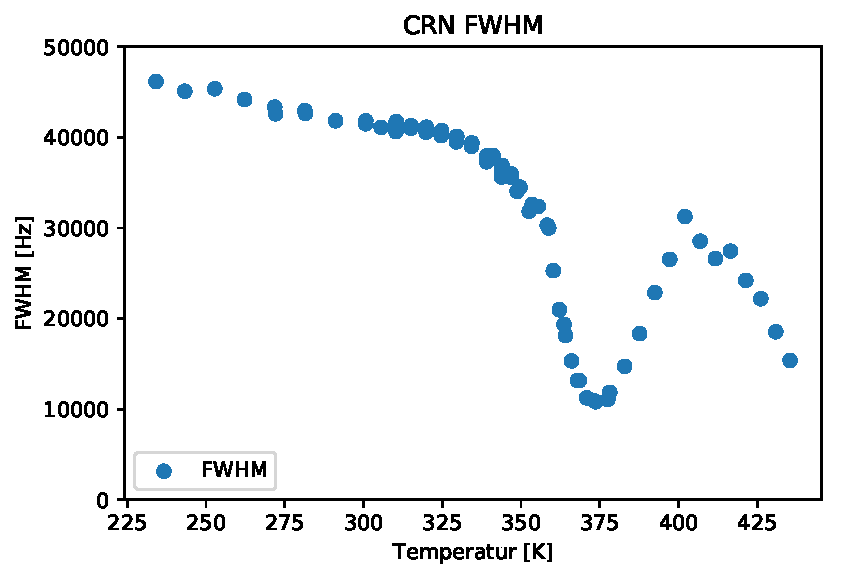
\includegraphics[width=\textwidth]{graphics/plots/SPEK/spek_fwhm.pdf}
	\end{center}
	\caption{Spektren FWHM} \label{fig:res:spek_fwhm}
\end{figure}
Um Beobachtungen zu quantisieren zwei Messgrößen: FWHM (Halbwertsbreite) und Schwerpunkt. Zwischen 350K und 360K sind die Spektren sehr verrauscht, ebenso bei 400K bis 420K; dort wurden Lorentz-Fits an die Spektren angelegt.

\begin{figure}
	\begin{center}
		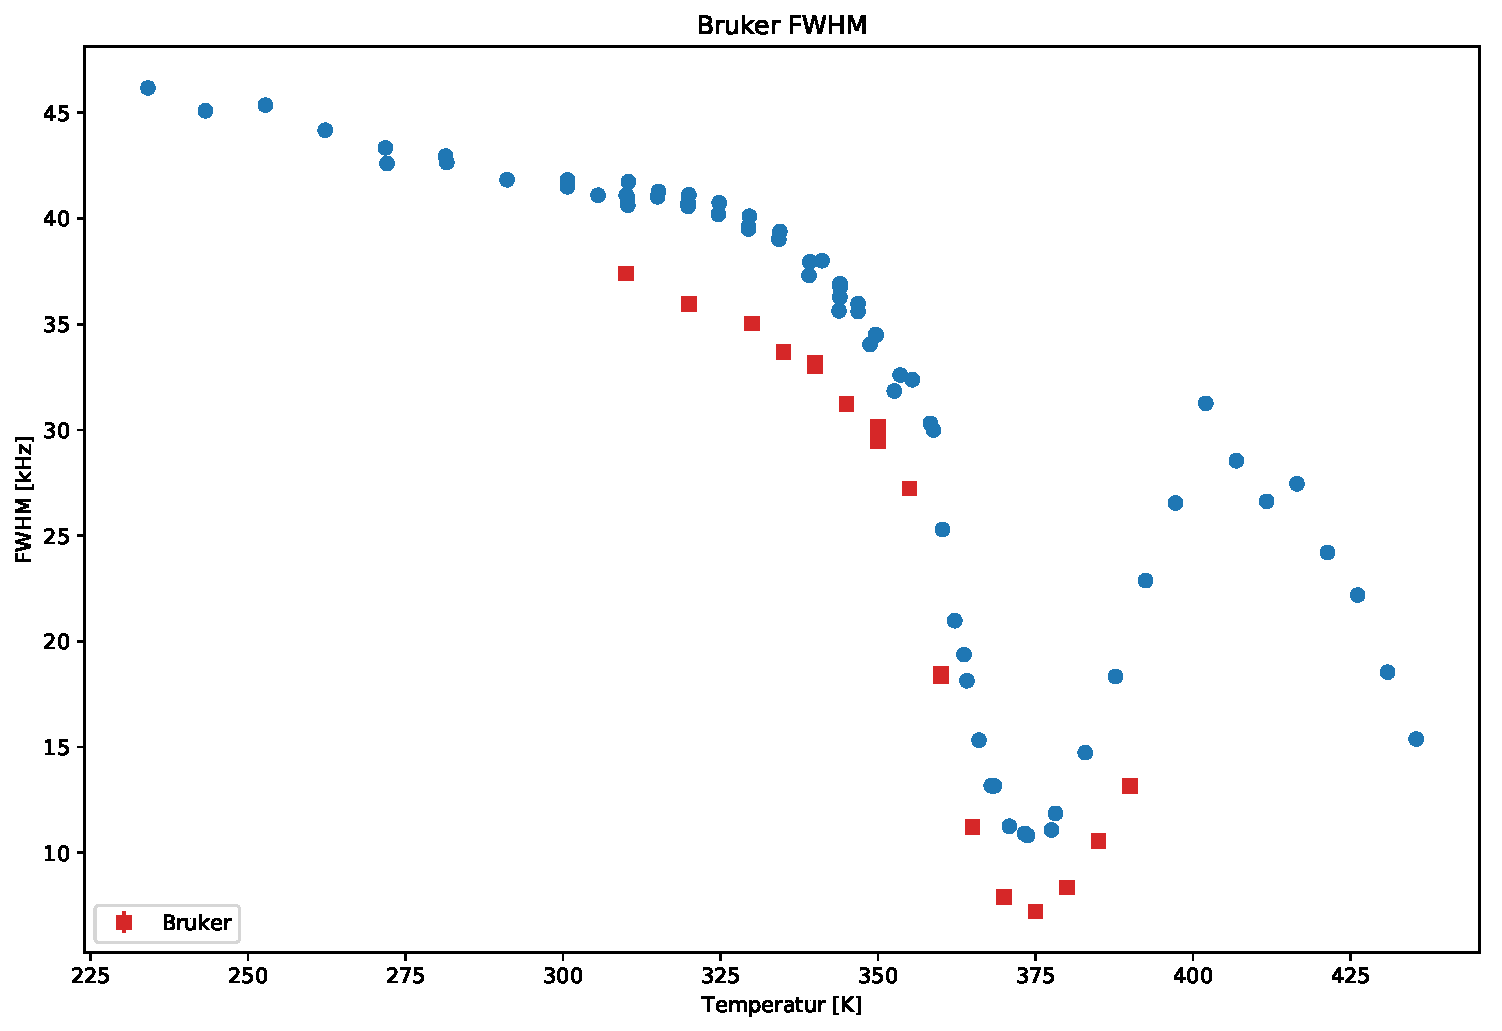
\includegraphics[width=\textwidth]{graphics/plots/BRUKER/bruker_fwhm.pdf}
	\end{center}
	\caption{Bruker FWHM} \label{fig:res:bruker_fwhm}
\end{figure}
Es gibt Abweichungen bei den Halbwertsbreiten. Es wäre aufgrund der Larmorfrequenzen (und der larmorfrequenzabhängigkeit des Quadrupol-WW) ein Verhältnis von 4:3 zu erwarten, was aber nicht ganz zutrifft. Messungen an einem $\SI{600}{MHz}$-Spektrometer wären hilfreich um Aussagen über die chemische Verschiebung machen zu können.


\begin{figure}
	\begin{center}
		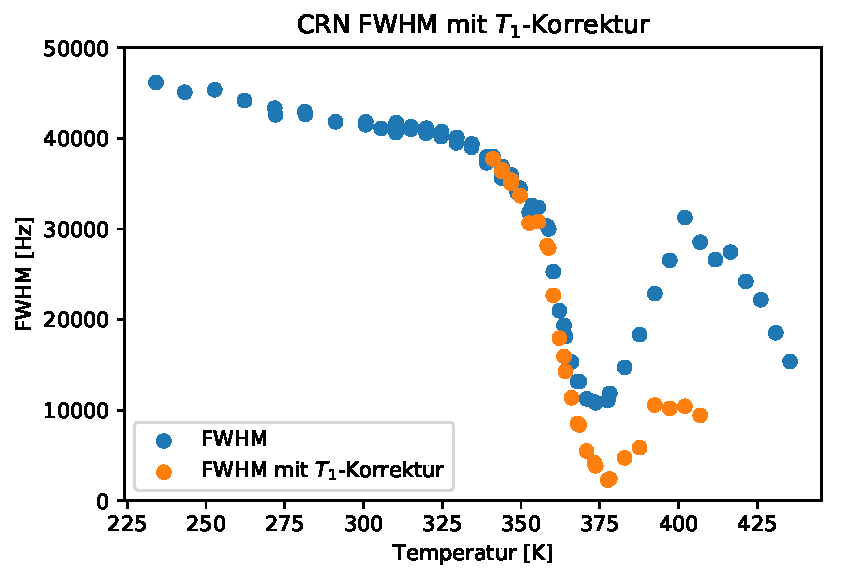
\includegraphics[width=\textwidth]{graphics/plots/SPEK/spek_t1korr.pdf}
	\end{center}
	\caption{Spektren FWHM mit $T_1$-Korrektur} \label{fig:res:spek_fwhm_t1}
\end{figure}
Aufgrund der Bewegungsverschmälerung würde man annehmen, dass die Halbwertsbreite sinkt, und nicht ein so hohes Maximum zeigt. Ein großer Einfluss ist die in dem Temperaturbereich (380K - 430K) sehr kurze $T_1$-Zeit. Durch den Einfluss von $T_1$ fällt das Signal sehr stark ab und verbreitert so das Spektrum.

Um den Einfluss von $T_1$ herauszurechnen: Die Spektren sind Fouriertransformierte der aufgenommenen Zeitsignale. Für die Spektren wird ein Lorentz 
\begin{align}
    L(f) = \frac{1}{\pi \gamma} \cdot \frac{\gamma^2}{\gamma^2 + (f - f_0)^2}
\end{align}
angenommen. Lorentz hat zwei Parameter, Maximum $f_0$ (und Schwerpunkt) und Halbwertsbreite $2\gamma$. Die Fouriertransformierte davon ist eine gedämpfte Schwingung:
\begin{align}
    h(t) = \exp{(-a |t|)} \cos{(2 \pi f_0 t)} \\
    H(t) = \int_{-\infty}^{\infty} h(t) \text{d} t \\
    H(f) = \frac{2}{a} \cdot \frac{(a/2\pi)^2}{((a/2\pi)^2) + (f - f_0)^2}
\end{align}
mit der Halbwertsbreite $2 \gamma = a/\pi$.

Das ursprüngliche Zeitsignal soll durch die $T_1$-Kurve geteilt werden, um den Einfluss herauszurechnen. Dafür werden ein Kohlrausch mit $\beta = 1$ angenommen, damit sich die Rechnung einfacher gestaltet:
\begin{align}
    f(t) = \exp{(-t/T_1)^\beta}
\end{align}
, die $T_1$-Werte stammen aus $T_1$-Messungen bei gleicher Temperatur. 

Fouriertransformiert ergibt sich die modifizierte Halbwertsbreite $2\gamma = 2(\gamma_0 - \frac{1}{\pi T_1})$.

Übrig bleibt ein kleinerer Peak (-> Theorie). Bei Temperaturen über 410K konnte keine Korrektur vorgenommen werden, weil die $T_1$-Werte da zu stark streuen.

\begin{figure}
	\begin{center}
		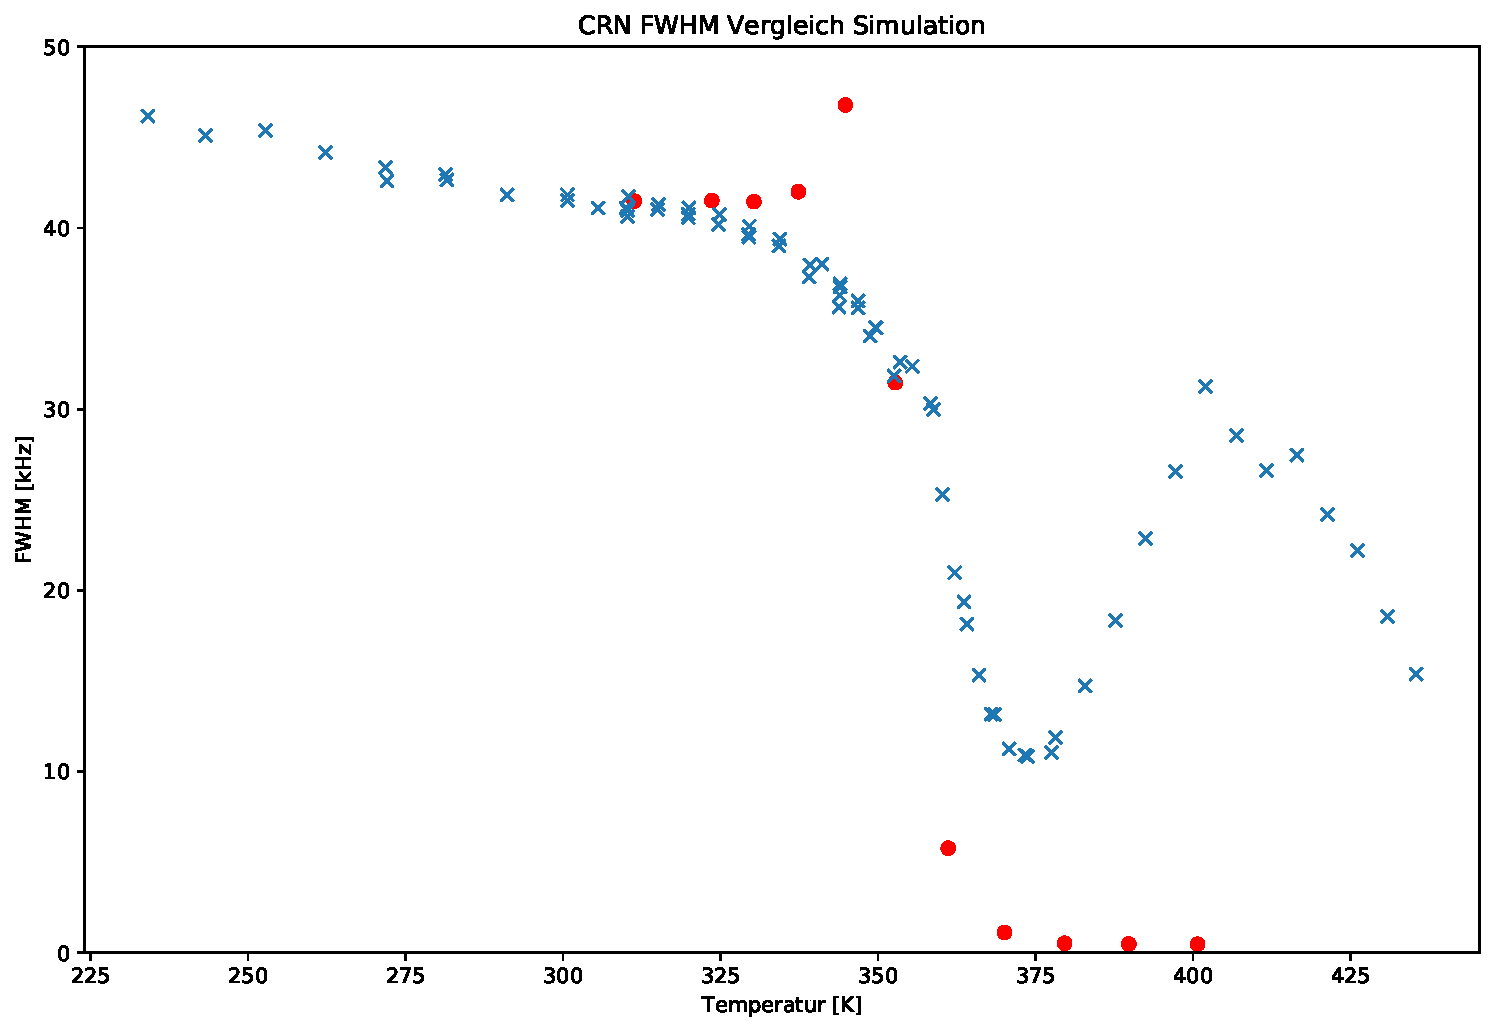
\includegraphics[width=\textwidth]{graphics/plots/SIM/sim_fwhm.pdf}
	\end{center}
	\caption{Simulation FWHM} \label{fig:res:sim_fwhm}
\end{figure}
Zusätzlich zeigt die Halbwertsbreite einen Peak bei ca. 350K. Dies kann daran liegen, dass hier der Übergang von der Czjzek-Form mit einer Spitze zur abgerundeten Lorentz-Form ist. Das Abrunden verschiebt die halbe Höhe zu niedrigeren Werten, daher der Peak. Die experimentellen Spektren zeigen aufgrund von Störungen auch bei niedrigeren keine perfekte Spitze und daher auch keinen Peak in der Halbwertsbreite beim Übergang.




\begin{figure}
	\begin{center}
		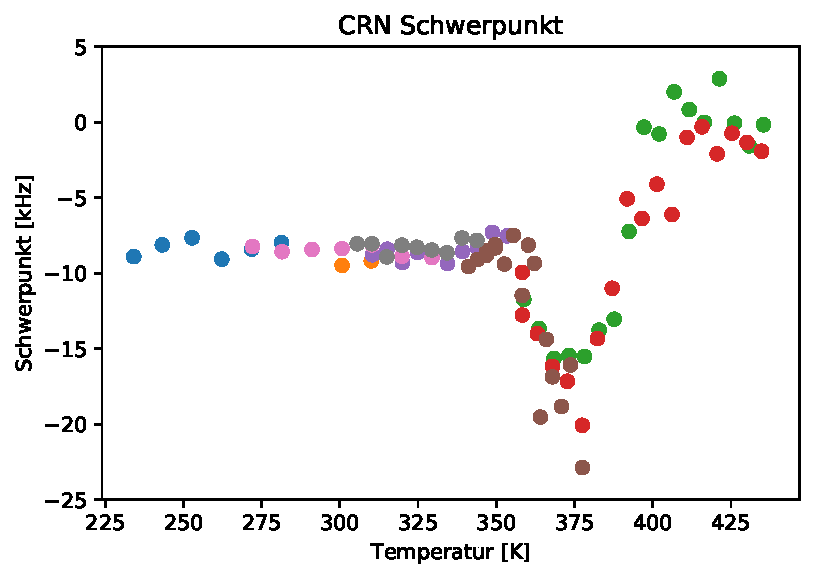
\includegraphics[width=\textwidth]{graphics/plots/SPEK/spek_mean.pdf} 
	\end{center}
	\caption{Spektren Schwerpunkt} \label{fig:res:spek_mean}
\end{figure}
Schwerpunkte; bei den stark verrauschten Spektren wurden die Werte wieder aus Lorentz-Fits bestimmt.

\begin{figure}
	\begin{center}
		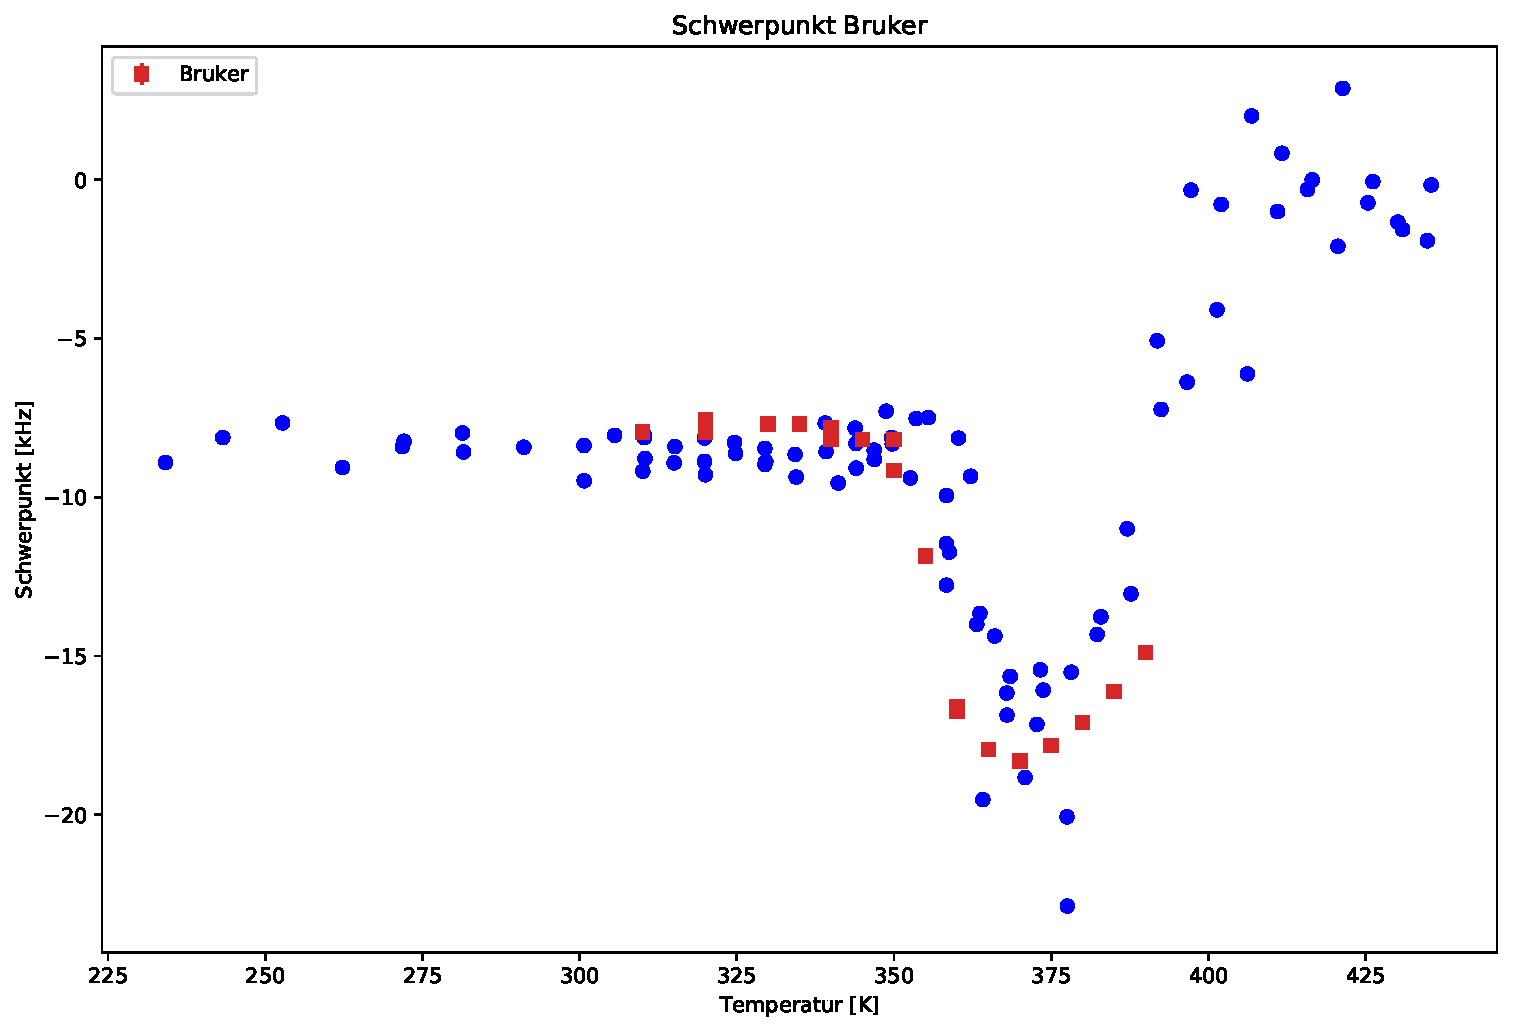
\includegraphics[width=\textwidth]{graphics/plots/BRUKER/bruker_mean.pdf} 
	\end{center}
	\caption{Bruker Schwerpunkt} \label{fig:res:bruker_mean}
\end{figure}


% \begin{figure} % ***
% 	\begin{center}
% 		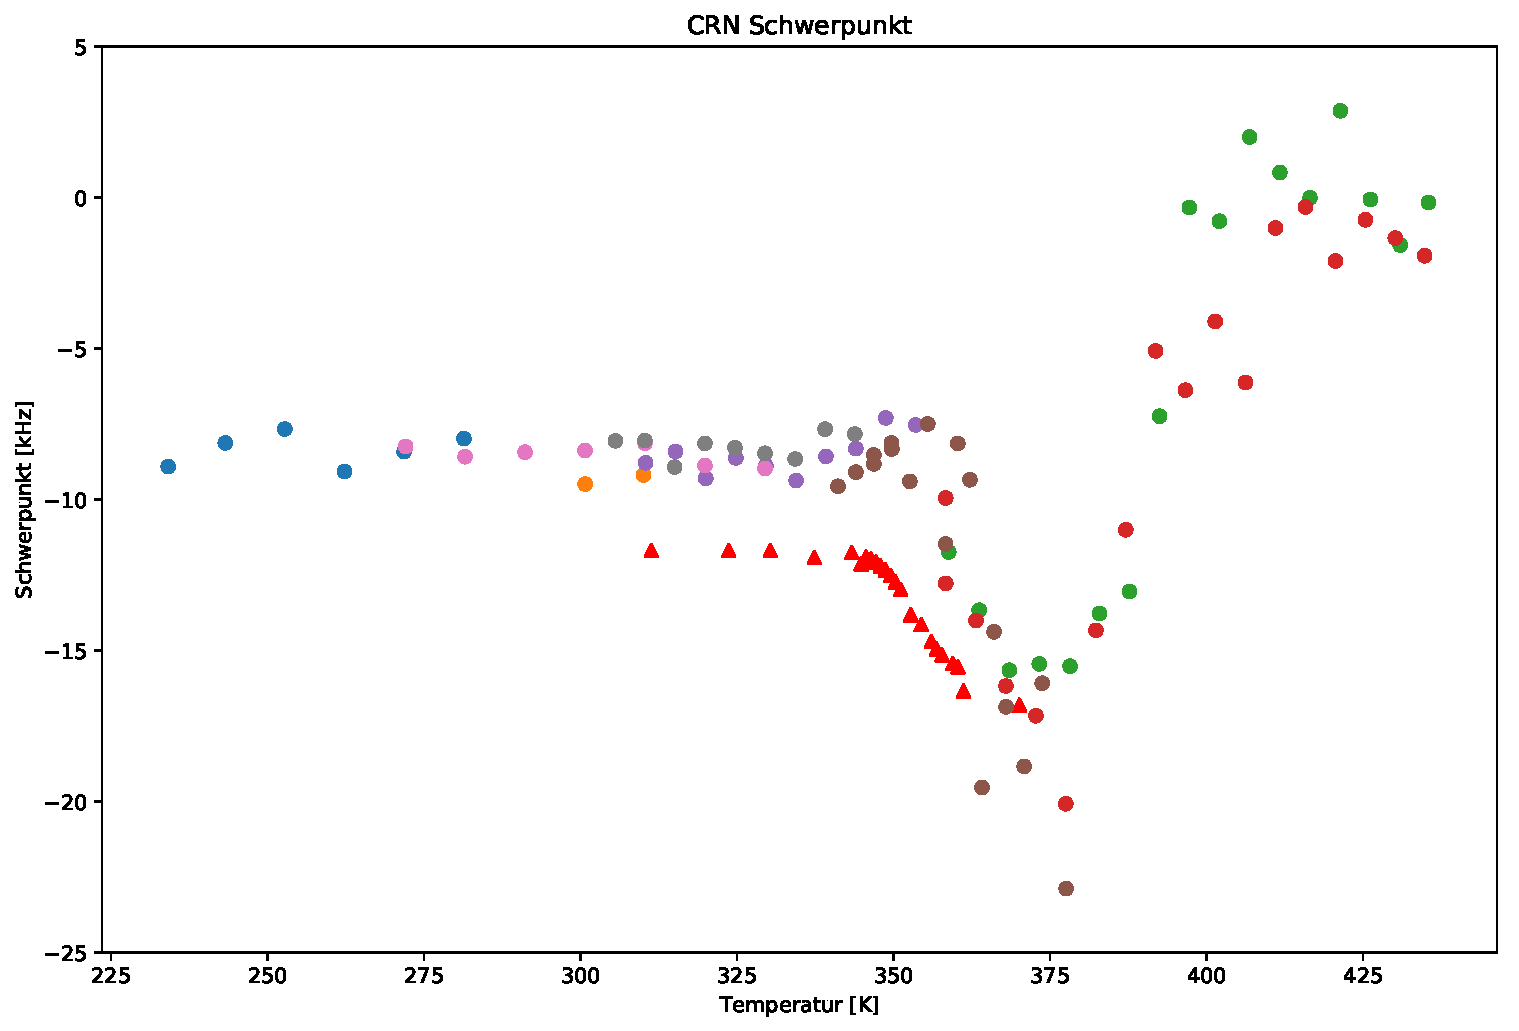
\includegraphics[width=\textwidth]{graphics/plots/SIM/sim_mean.pdf} 
% 	\end{center}
% 	\caption{Simulation Schwerpunkt} \label{fig:res:sim_mean}
% \end{figure}

















\section{Theorie} \label{section:res:theorie}

Die experimentellen Ergebnisse sollen mit den theoretischen Überlegungen vergleichen werden.

\begin{figure}
	\begin{center}
		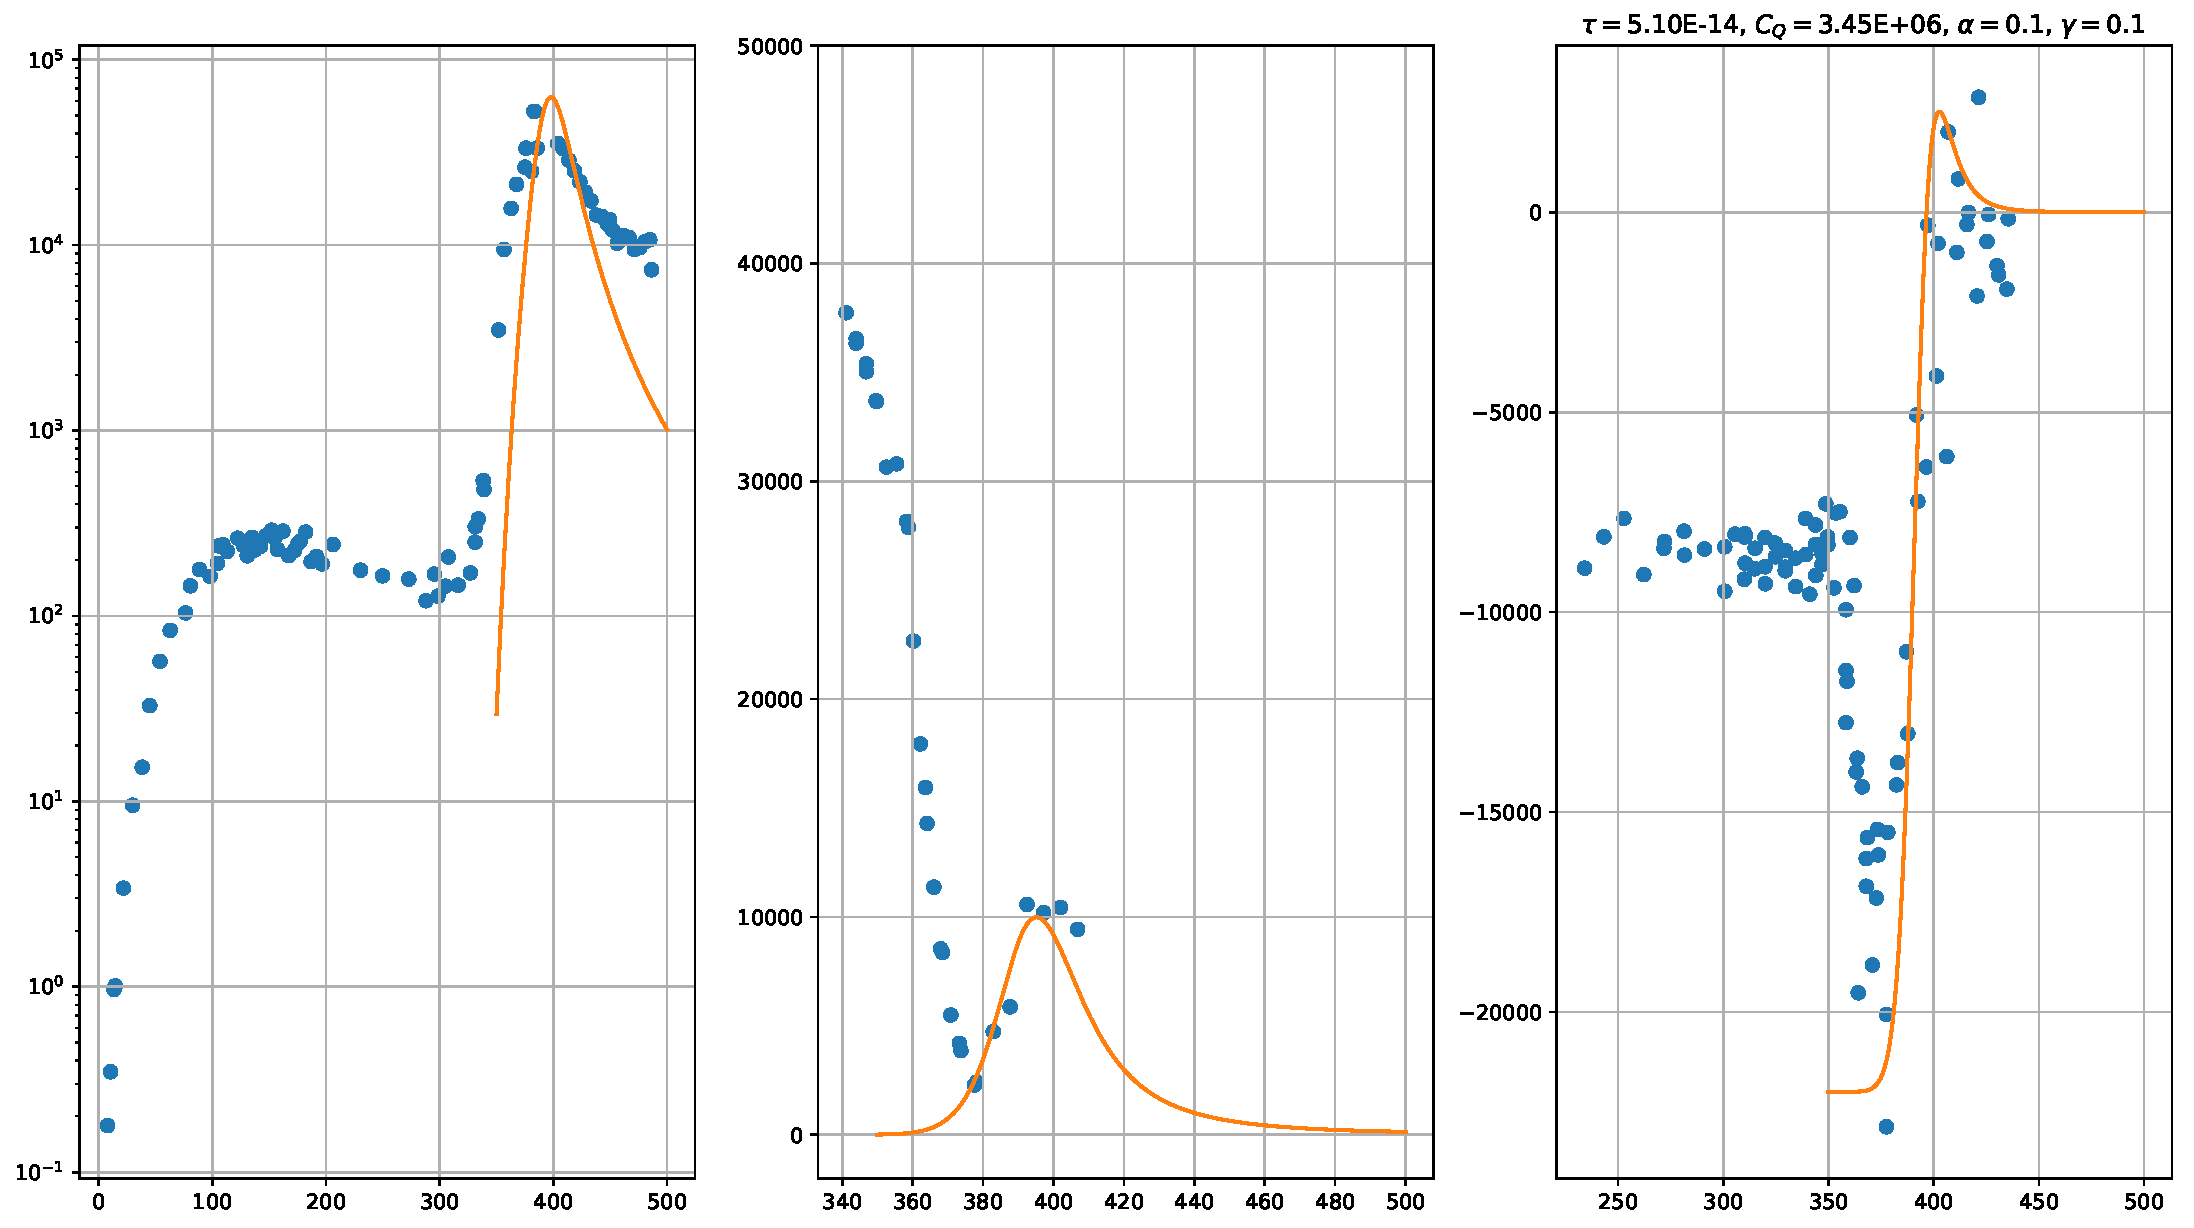
\includegraphics[width=\textwidth]{graphics/plots/THEO/J_01.pdf}
	\end{center}
	\caption{Spektraldichte $J$} \label{fig:res:theorie_j}
\end{figure}
Es werden verschiedene Spektraldichten verwendet, hier zuerst BPP. $\tau_c$ stammt aus dem 4er-Papier.

Für $C_Q = \SI{3.45}{MHz}$ gibt es eine gute Übereinstimmung für die $T_1$-bereinigte Halbwertsbreite und den Schwerpunkt, bei $T_1$ stimmt die grobe Form, bei den Flanken gibt es starke Abweichungen.

Mit $J_{CC}$ lässt sich mit $C_Q = \SI{3.65}{MHz}$ und $\alpha = 0.64$ $T_1$ gut abbilden, aber es gibt große Abweichungen bei der Halbwertsbreite. 

$J_{DC}$ ist mit $C_Q = \SI{3.2}{MHz}$ und $\gamma = 1.12$ ein Kompromiss in die andere Richtung, Schwerpunkt und Halbwertsbreite scheinen zu passen, aber bei $T_1$ gibt es wieder Abweichungen. 

Bei den Schwerpunkten von $J_{CC}$ und $J_{DC}$ ist noch zu klären, ob die verwendete Funktion für den Imaginärteil der Spektraldichte korrekt ist.

Alle drei Spektraldichten zeigen zwar gute, aber keine perfekten Übereinstimmungen mit den experimentellen Daten.



\begin{figure}
	\begin{center}
		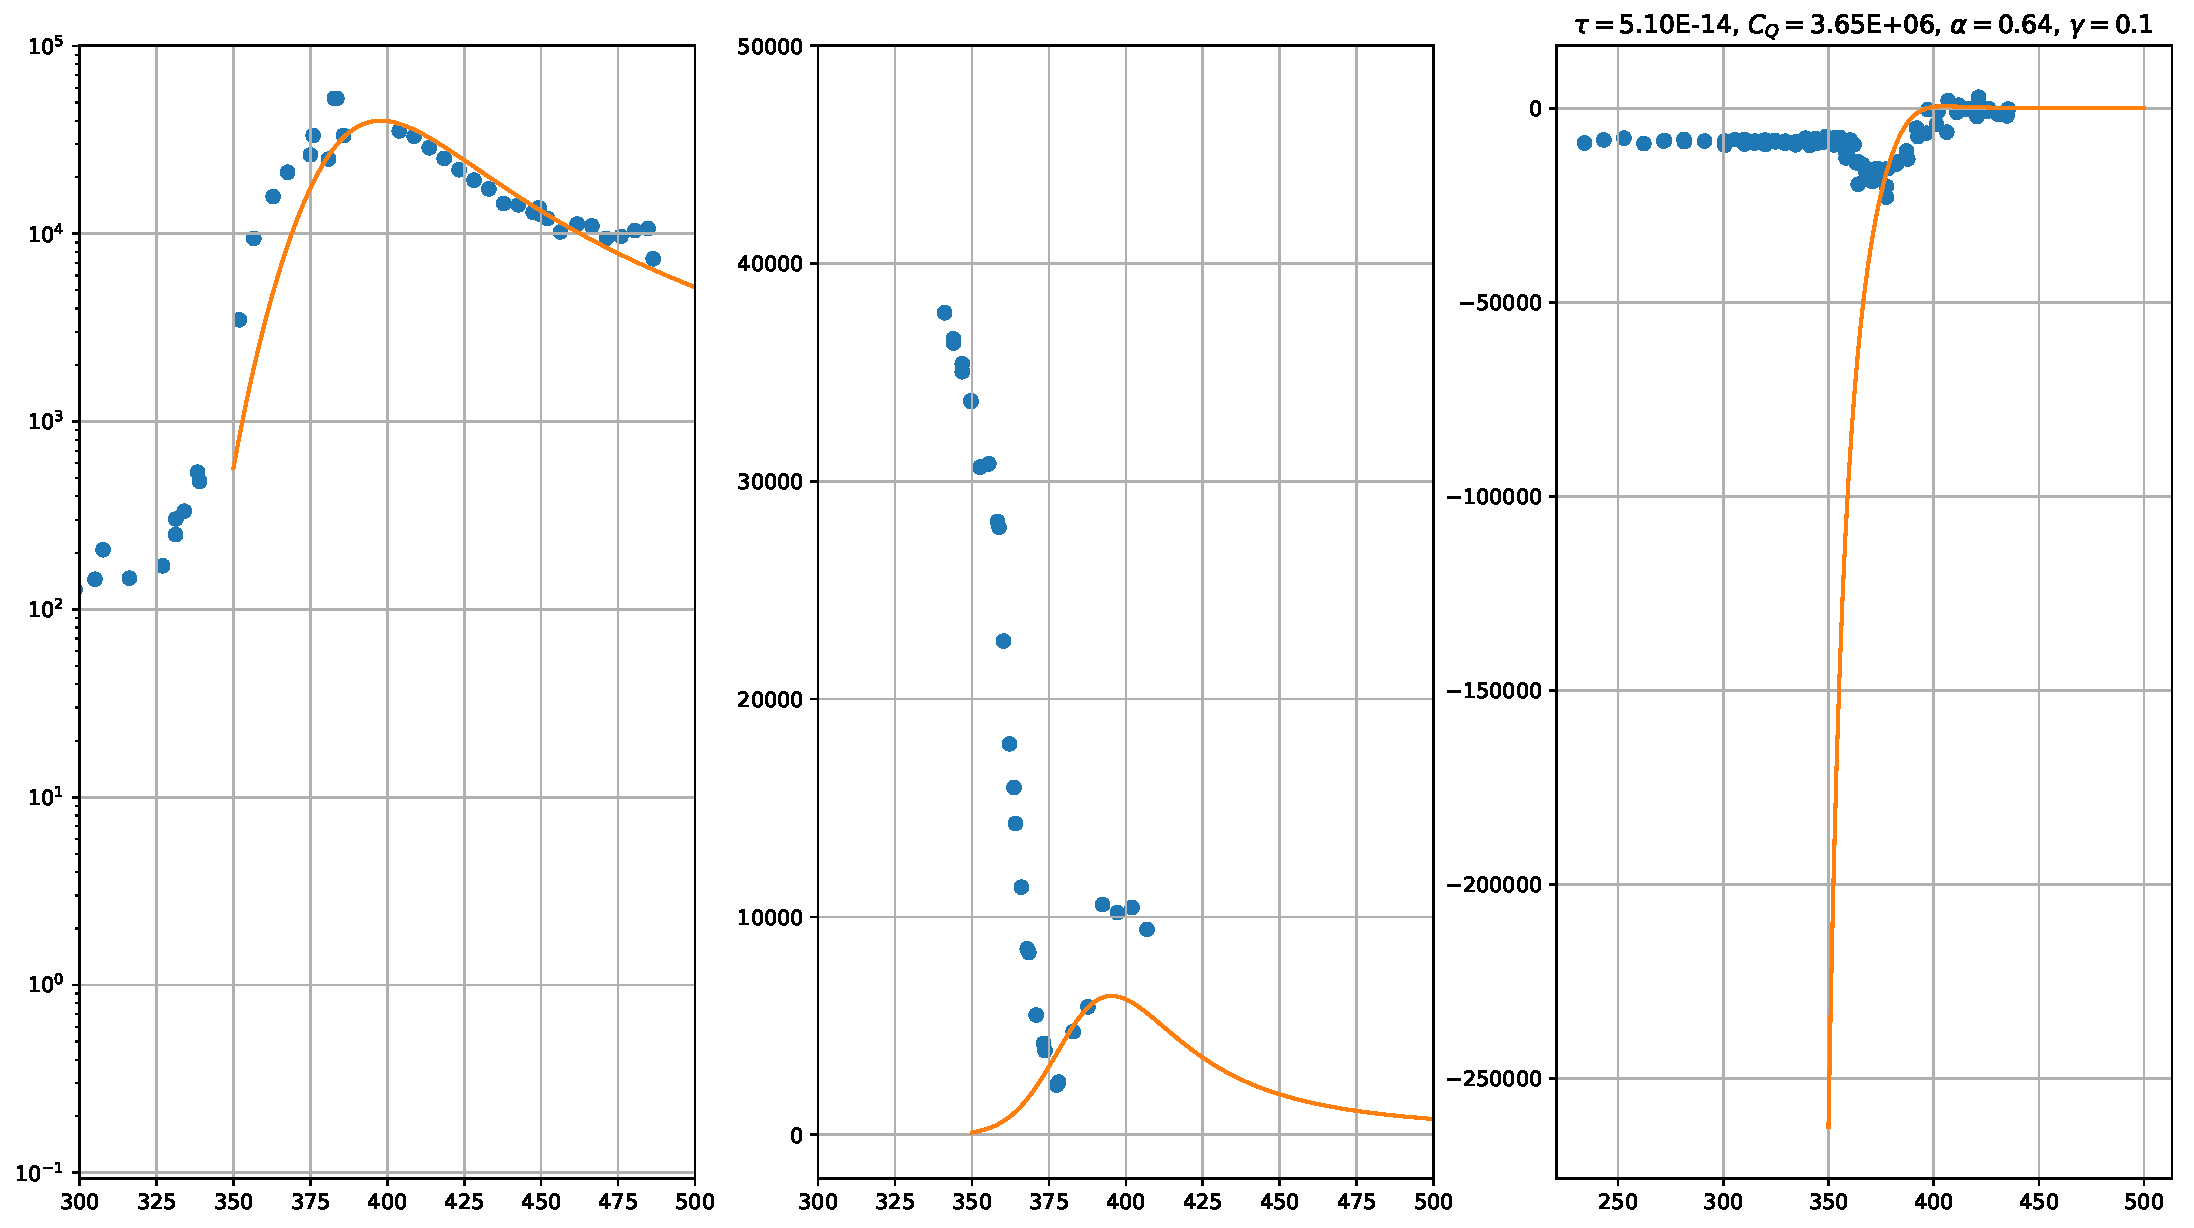
\includegraphics[width=\textwidth]{graphics/plots/THEO/J_cc_02.pdf}
	\end{center}
	\caption{Spektraldichte $J_{CC}$} \label{fig:res:theorie_j_cc}
\end{figure}

\begin{figure}
	\begin{center}
		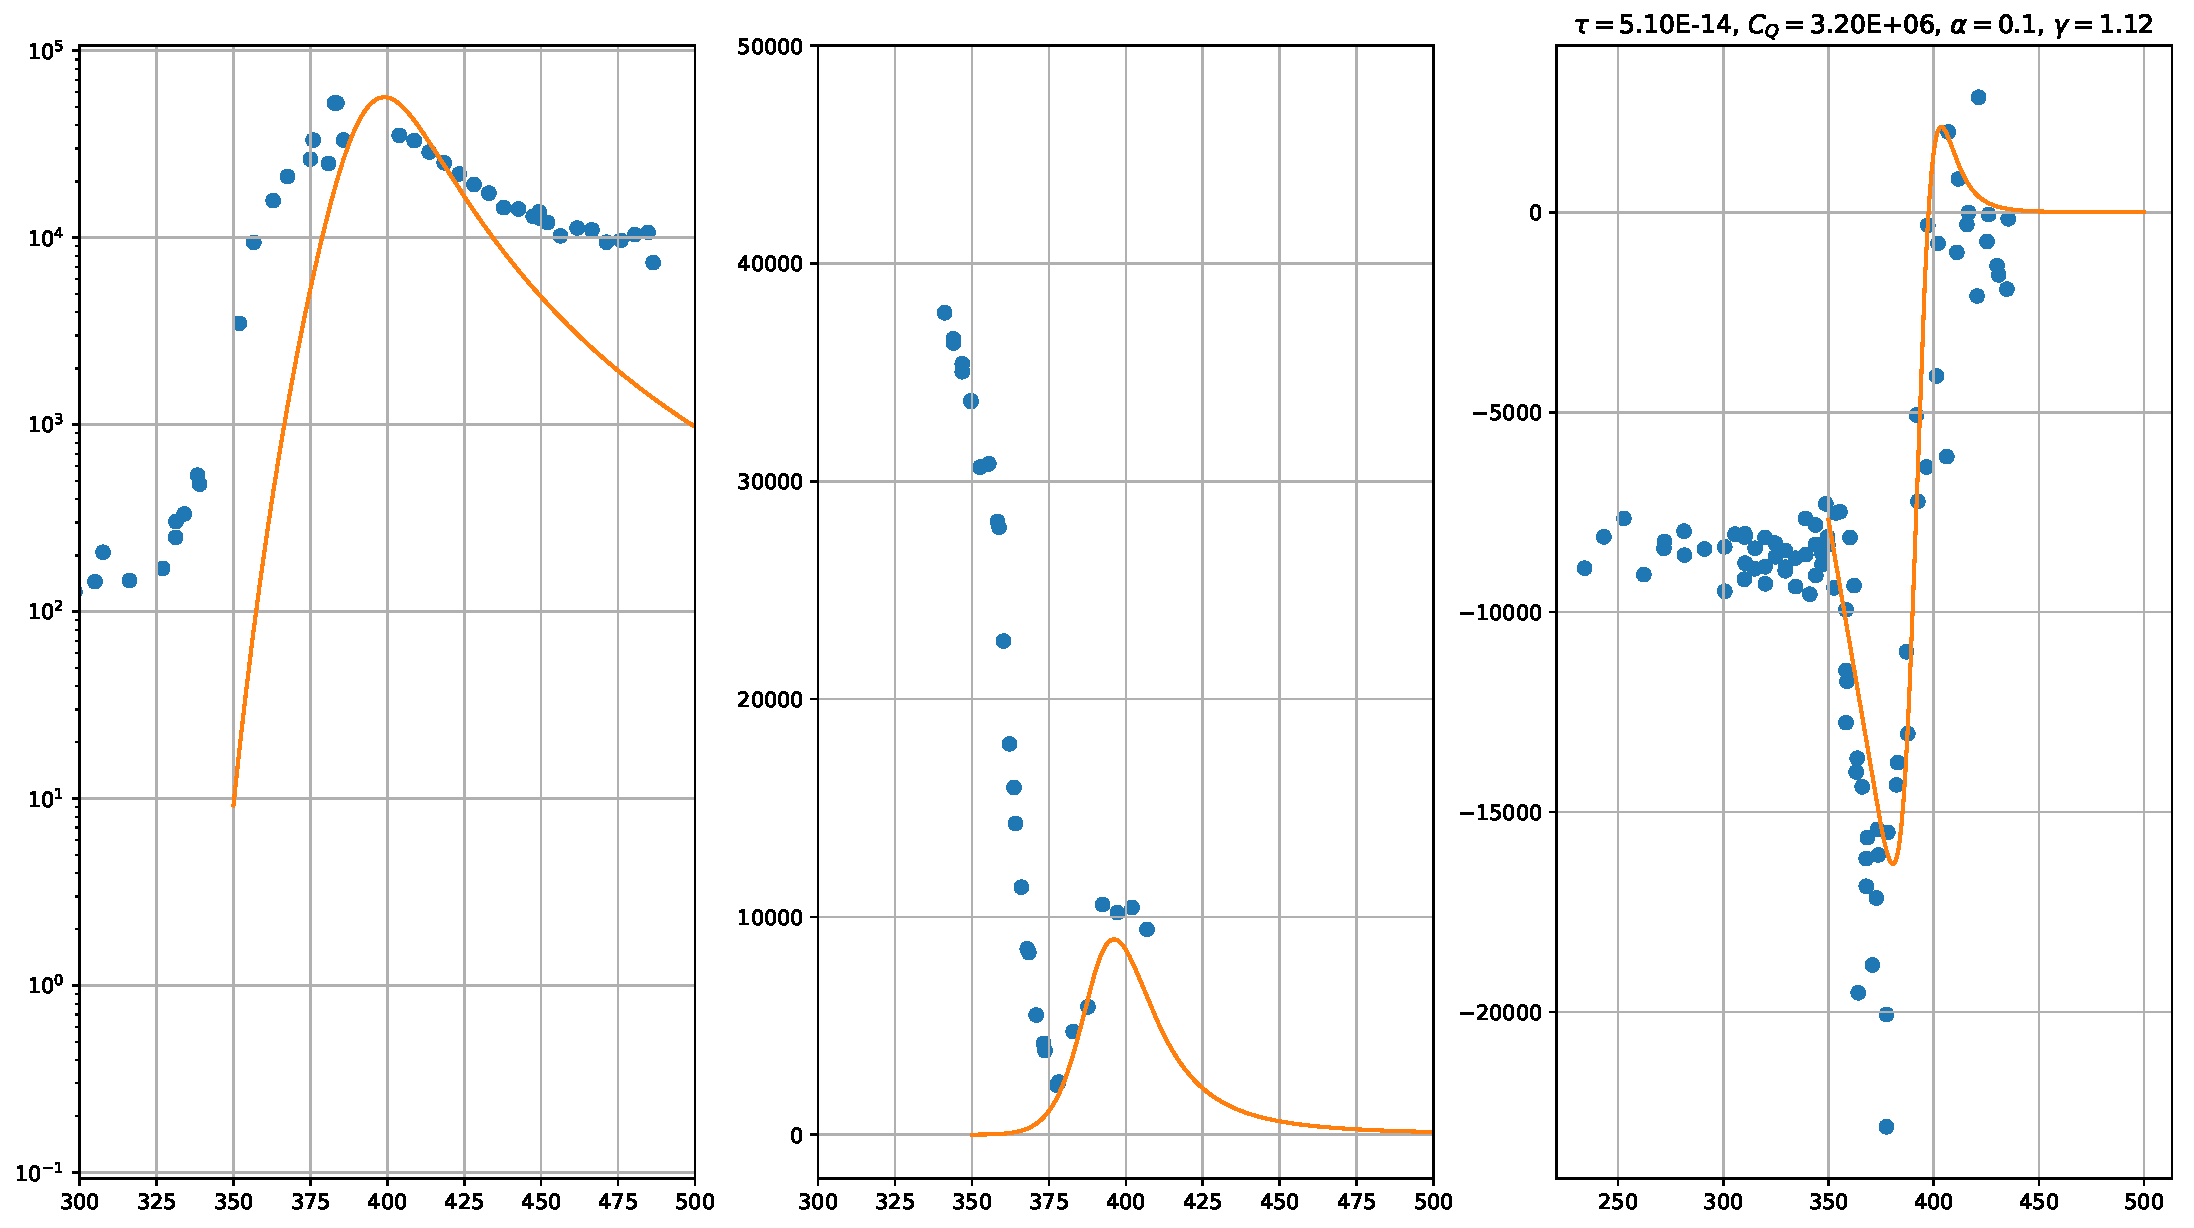
\includegraphics[width=\textwidth]{graphics/plots/THEO/J_dc_01.pdf}
	\end{center}
	\caption{Spektraldichte $J_{DC}$} \label{fig:res:theorie_j_dc}
\end{figure}



\section{Theoretische Beschreibung experimenteller CRN-Daten} \label{section:theo:daten}


Es wurde untersucht, ob vorliegende gemessenen Daten mit den beschriebenen Theorien in Einklang gebracht werden können. Dafür wurden die Daten zu $T_1$, zu Spektren untersucht; die $T_1$-Daten stammen dabei aus Messungen von C. Zürn \cite{zuern_paper} an einer 2Ca(NO$_3$)$_2$-3RbNO$_3$-Probe, während alle weiteren Daten mit der von Zürn verwendeten Probe im Rahmen dieser Masterarbeit aufgenommen wurden.

Um eine Übereinstimmung zur Theorie feststellen zu können, müssen sich alle Datensätze mit dem gleichen Satz geteilter Parameter beschreiben lassen. Im Falle der Spektraldichte $J(\omega)$ sind dies $C_Q$ und $\tau_{co}$; für $J_{CC}$ und $J_{CD}$ sind $\alpha$ bzw. $\gamma$ zusätzliche Parameter.

Nach \cite{PIMENOV199793} wird für CRN für die Korrelationszeit ein Vogel-Fulcher-Gesetz
\begin{align}
	\tau_c = \tau_{co} \exp \left( \frac{D T_\text{VF}}{T-T_\text{VF}} \right) 
\end{align}
mit dem strength index $D = \SI{3.5}{}$, der Vogel-Fulcher-Temperatur $T_\text{VF} = \SI{294}{K}$ und dem Frequenzfaktor $\tau_{co} = \SI{5.1e-14}{s}$ (der beim Vergleich mit den Daten dennoch als freier Parameter angesehen werden soll um dem Fit eine größtmögliche Flexibilität zu erlauben) angenommen.

\begin{wrapfigure}{r}{0.5\textwidth}
	\vspace{-20pt}
	\begin{center}
		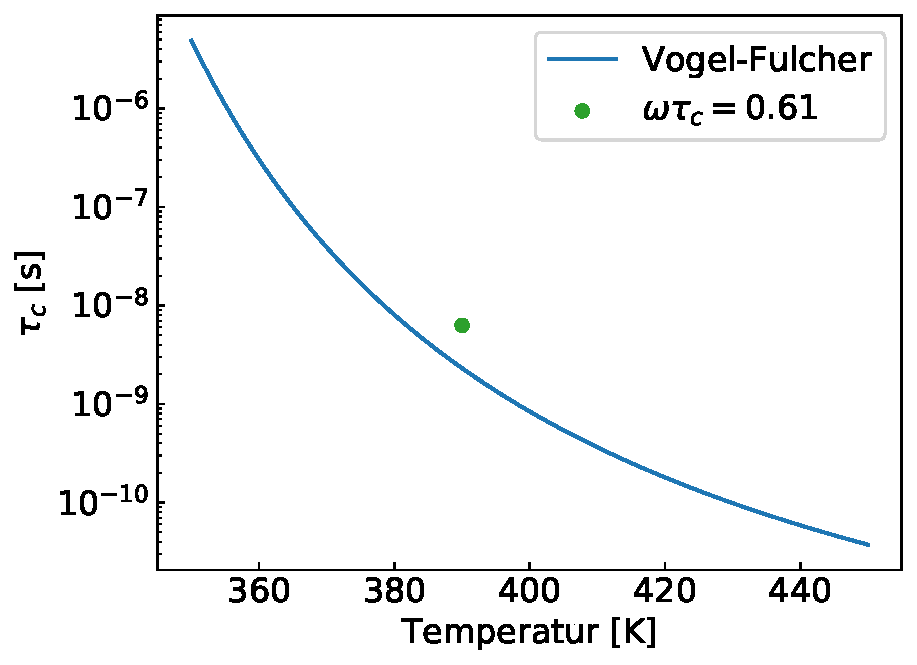
\includegraphics[width=0.49\textwidth]{graphics/zwischenbericht/tau_c_arrhenius_vogel_fulcher.pdf}
	\end{center}
	\vspace{-20pt}
	\caption{Vergleich von Korrelationszeiten basierend auf Vogel-Fulcher-Gesetz \label{fig:korrelationszeiten}}
\end{wrapfigure}
Am $T_1$-Minimum nach Gleichung \eqref{eqn:bpp} gilt $\omega \tau_c \approx \SI{0.61}{}$ \cite[S. 629]{omegatau061}. Das $T_1$-Minimum kann in den Daten bei etwa $T_\text{min} = \SI{390}{K}$ gefunden werden; die Larmorfrequenz liegt bei $\omega_L = \SI{97.1722}{MHz}$, was bedeutet, dass bei $T_\text{min}$ gilt $\tau_c \approx \frac{\SI{0.61}{}}{\omega_L} \approx \SI{6.28}{\nano s}$. Vergleicht man das Vogel-Fulcher-Gesetz mit diesem Punkt, lässt sich erkennen, dass eine gute Übereinstimmung vorliegt.


Die aufgenommenen Daten unterstützen eine biexponentielle Interpretation wie in \eqref{eqn:trans_relax} nur schwerlich, daher wurde lediglich der deutlich zu beobachtende Anteil des Zentralübergangs, $\Delta_c$ und $\omega_c^{(2)}$, für die entsprechenden FWHM- bzw. Schwerpunkts-Daten betrachtet. Für die $T_1$-Daten wird Formel \eqref{eqn:bpp} verwendet. Um einen Ausgangspunkt für die Analyse zu schaffen, wurden alle Fits per Hand erstellt, wobei durch das Ändern der Parameter versucht wurde eine möglichst gute Übereinstimmung zu erreichen.

Für die Spektraldichte $J(\omega)$ kann, wie in Abbildung \ref{fig:triple_vergleich} zu sehen, mit $\eta^2 = 42 - 24 \sqrt{3} \approx \SI{0.43}{}$ \cite{caer} und den Parametern $C_Q = \SI{3e6}{Hz}$ und $\tau_c = \SI{3.9e-14}{s}$ eine vergleichsweise gute Übereinstimmung für die $T_1$-Werte erreicht werden, die Flanken unterscheiden sich jedoch deutlich. Die Abweichungen der FWHM-Werten und der Schwerpunkte sind mit einem Faktor von etwa 4 bzw. etwa 2 bedeutend.
\begin{figure}[htbp]
	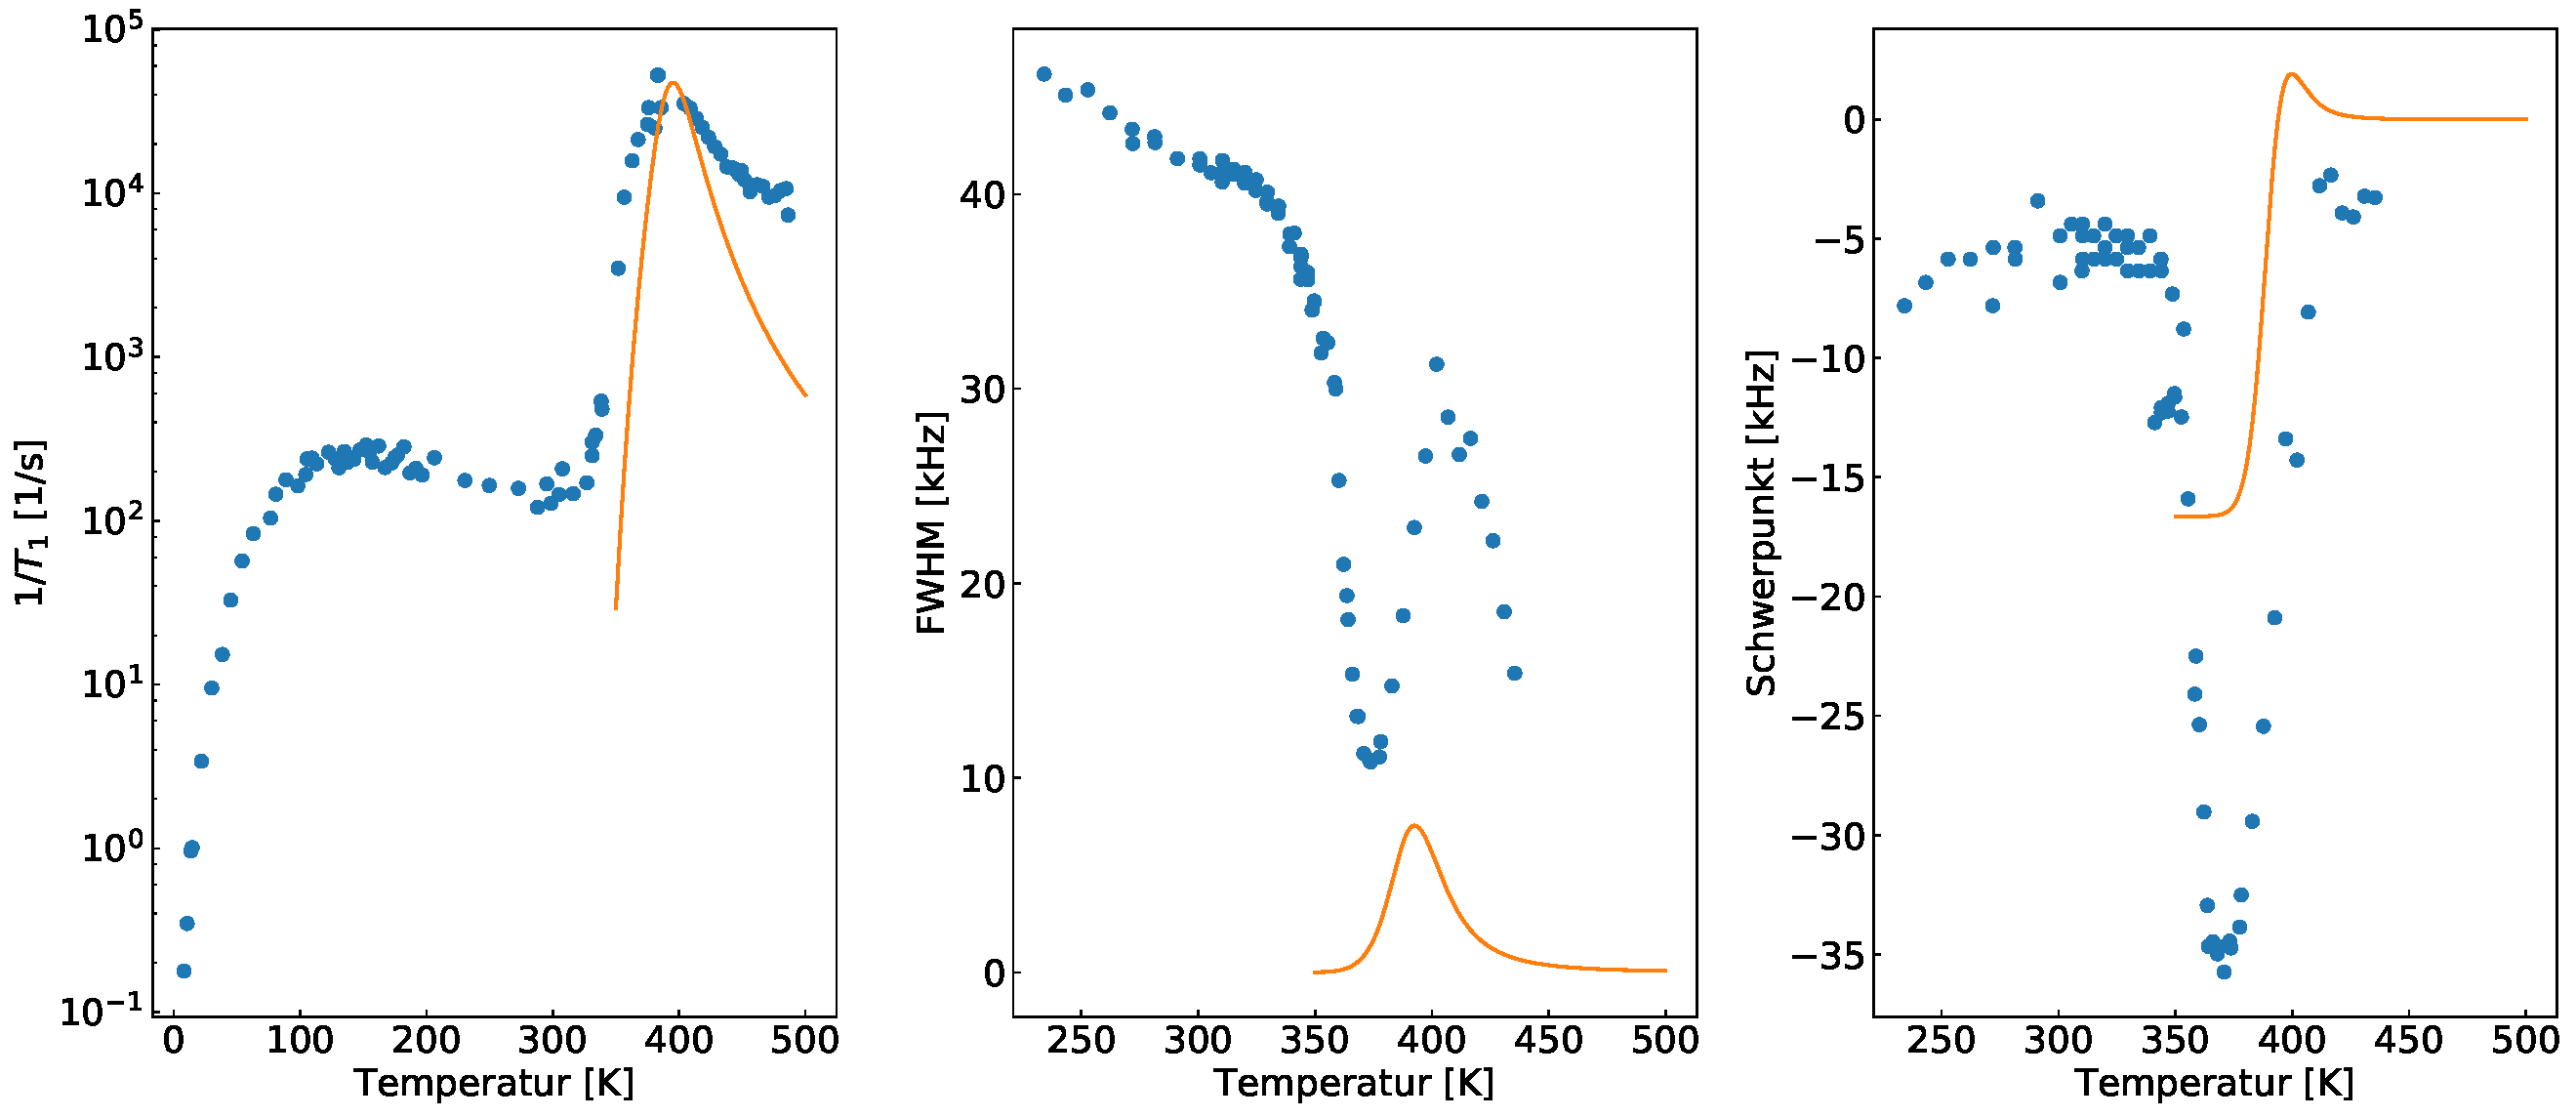
\includegraphics[width=\textwidth]{graphics/zwischenbericht/J_fertig.pdf}
	\caption{Vergleich der $T_1$-, FWHM- und Schwerpunkts-Daten (in blau) und der angepassten Theoriekurven (in orange). \label{fig:triple_vergleich}}
\end{figure}

Eine mögliche Erklärung für die Abweichung der FWHM-Werte könnte sein, dass in diesem Fall nicht, wie nach Formel \eqref{eqn:fwhm}, nur $T_2$, sondern auch das bei Temperaturen um $\SI{400}{K}$ mit etwa $\SI{50}{\micro s}$ äußerst kurze $T_1$ zur Verbreiterung des Spektrums und damit zu dessen FWHM-Werten beiträgt. Erste Versuche, den Effekt der $T_1$-Relaxation aus dem Spektrum herauszurechnen, scheinen vielversprechend. Für die Abweichungen der Schwerpunkts-Daten von der Theorie steht eine entsprechende Erklärung noch aus.

Aus diesem Grund jedoch soll für die Spektraldichten $J_{CC}$ und $J_{CD}$ die FWHM-Werte zunächst nicht betrachtet werden. Gleiches gilt für den Schwerpunkt, da die entsprechenden Imaginärteile der Spektraldichten, $Q_{CC}$ und $Q_{CD}$, nicht zur Verfügung stehen.

Für die Parameter $C_Q = \SI{2.85e6}{Hz}$, $\tau_c = \SI{7e-15}{s}$ und $\alpha = \SI{0.38}{}$ kann mit der Spektraldichte $J_{CC}$ in diesem Temperaturbereich eine noch bessere Übereinstimmung zu den $T_1$-Daten erzielt werden, für die Parameter $C_Q = \SI{2.7e6}{Hz}$, $\tau_c = \SI{4.4e-14}{s}$ und $\gamma = \SI{0.66}{}$ erreicht die Spektraldichte $J_{CD}$ eine leicht bessere Übereinstimmung als die Spektraldichte $J$; die entsprechenden Plots sind in Abbildung \ref{fig:j_cc_j_cd} zu finden.
\begin{figure}[H]
	\centering
	\begin{subfigure}{0.49\textwidth}
		\centering
		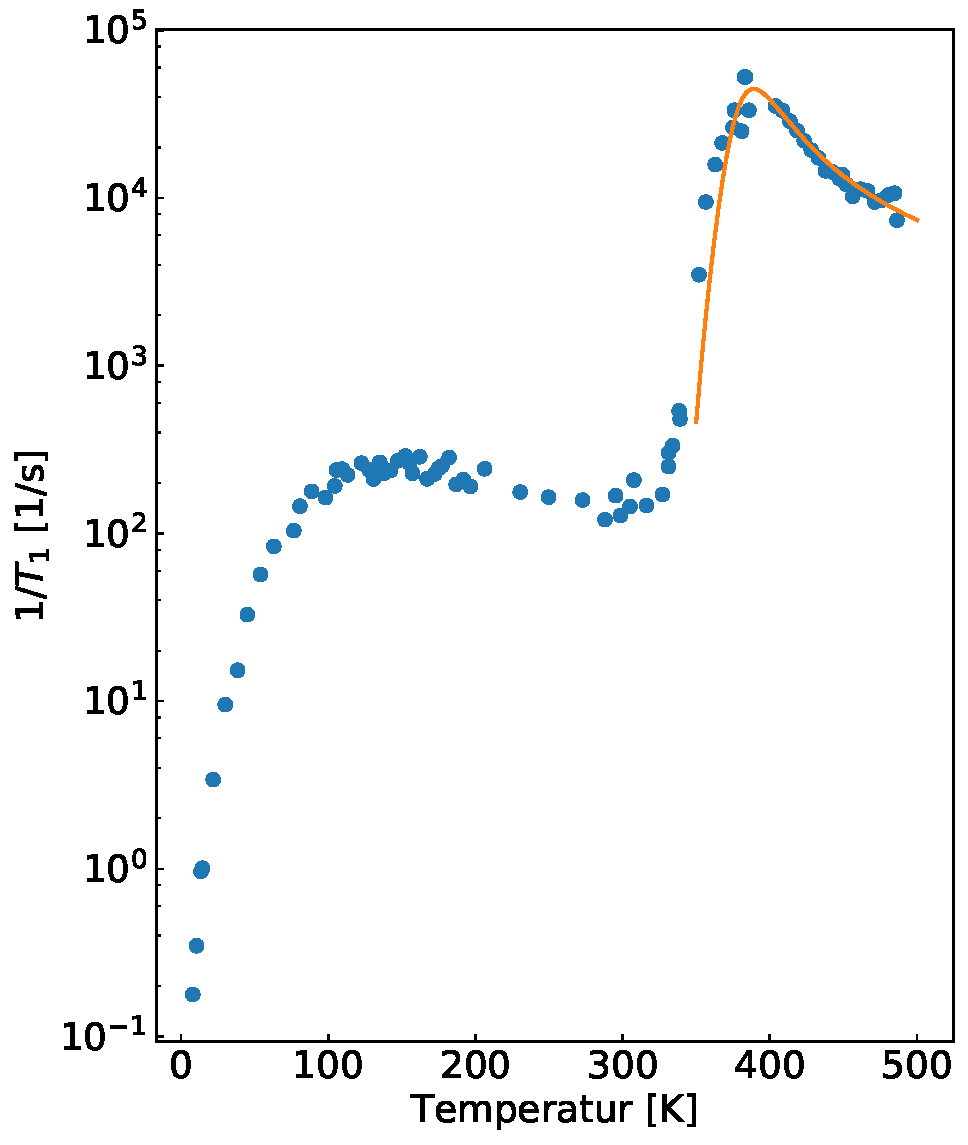
\includegraphics[width=0.95\textwidth]{graphics/zwischenbericht/J_cc.pdf}
	\end{subfigure}%
	\begin{subfigure}{0.49\textwidth}
		\centering
		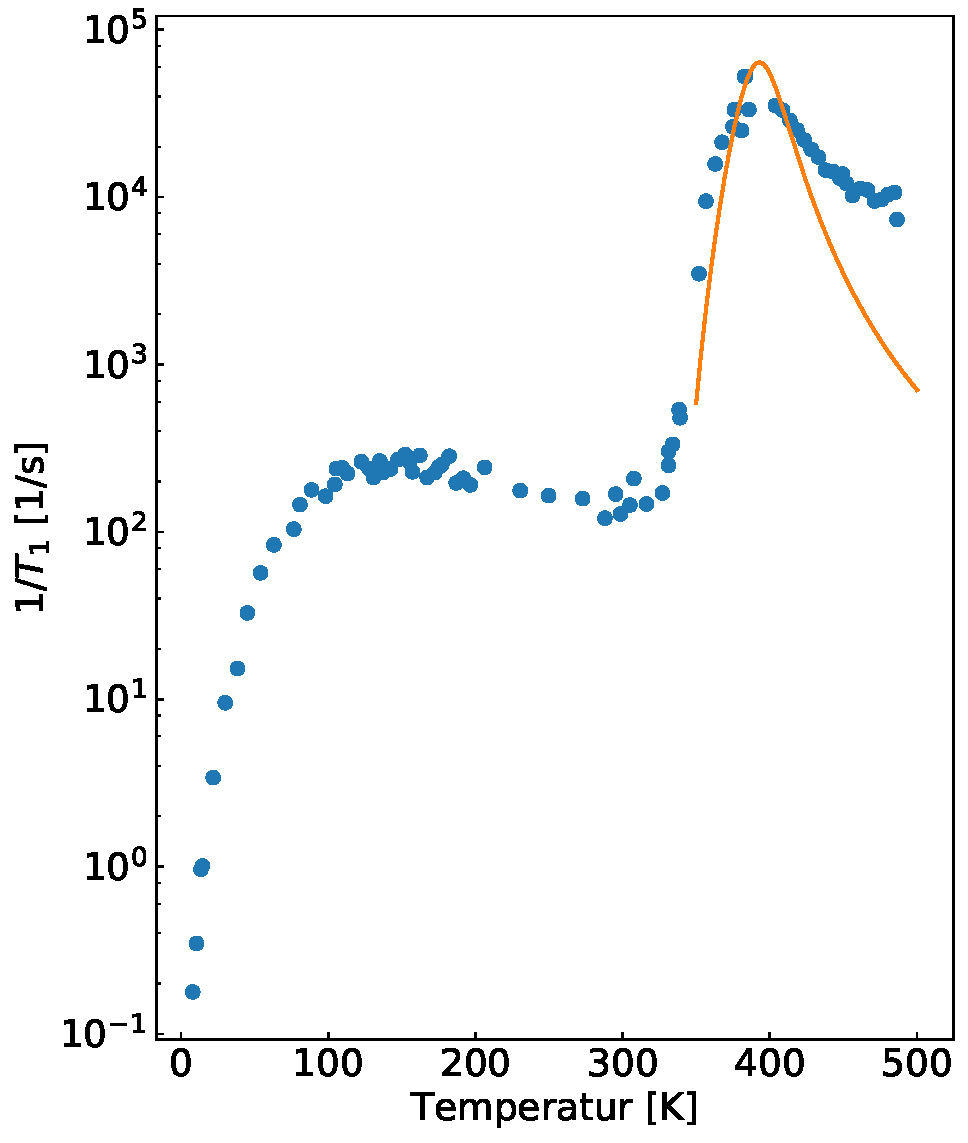
\includegraphics[width=0.95\textwidth]{graphics/zwischenbericht/J_cd.pdf}
	\end{subfigure}
	\caption{Spektraldichten $J_{CC}$ (links) und $J_{CD}$ (rechts), angepasst an die Daten}
	\label{fig:j_cc_j_cd}
\end{figure}

Die nächsten Schritte in dieser Untersuchung sollen darin bestehen, die Auswirkungen der $T_1$-Relaxation auf die Spektrums-Breite zu bestimmen und schlussendlich zu ergründen, ob sich die Messdaten sich mit diesen Theorien zufriedenstellend erklären lassen.




Werden die resultierenden Zeitkonstanten zusammen mit $T_2$ aufgetragen, zeigt sich eine hohe Ähnlichkeit, was vermuten lässt, dass mit der Methode $T_2$ gemessen wurde.
\begin{figure}
	\begin{center}
		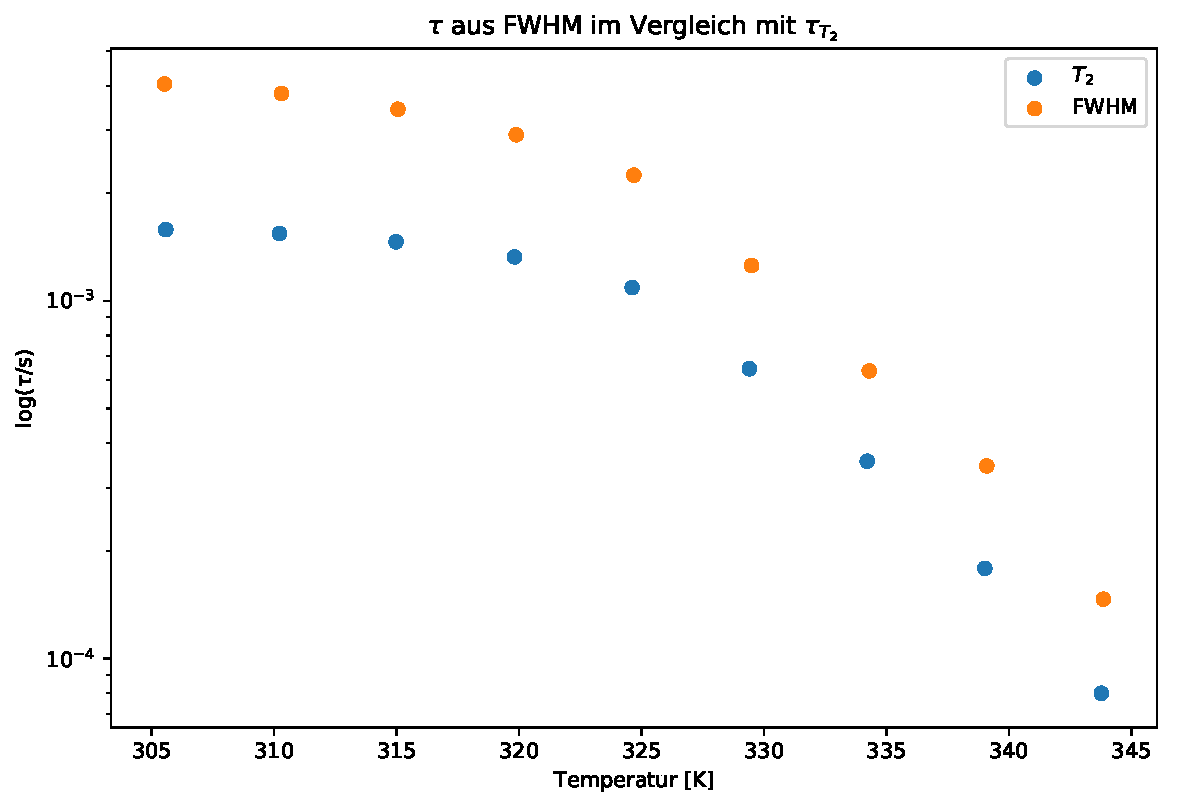
\includegraphics[width=\textwidth]{graphics/plots/SPEKDYN/spekdyn_t2.pdf}
	\end{center}
	\caption{$\tau$ aus FWHM im Vergleich mit $T_2$} \label{fig:res:spekdyn_t2}
\end{figure}
